\documentclass[]{ctexbook}
\usepackage{lmodern}
\usepackage{amssymb,amsmath}
\usepackage{ifxetex,ifluatex}
\usepackage{fixltx2e} % provides \textsubscript
\ifnum 0\ifxetex 1\fi\ifluatex 1\fi=0 % if pdftex
  \usepackage[T1]{fontenc}
  \usepackage[utf8]{inputenc}
\else % if luatex or xelatex
  \ifxetex
    \usepackage{xltxtra,xunicode}
  \else
    \usepackage{fontspec}
  \fi
  \defaultfontfeatures{Ligatures=TeX,Scale=MatchLowercase}
\fi
% use upquote if available, for straight quotes in verbatim environments
\IfFileExists{upquote.sty}{\usepackage{upquote}}{}
% use microtype if available
\IfFileExists{microtype.sty}{%
\usepackage{microtype}
\UseMicrotypeSet[protrusion]{basicmath} % disable protrusion for tt fonts
}{}
\usepackage[b5paper,tmargin=2.5cm,bmargin=2.5cm,lmargin=3.5cm,rmargin=2.5cm]{geometry}
\usepackage[unicode=true]{hyperref}
\PassOptionsToPackage{usenames,dvipsnames}{color} % color is loaded by hyperref
\hypersetup{
            pdftitle={Face lab book},
            pdfauthor={Face lab},
            colorlinks=true,
            linkcolor=Maroon,
            citecolor=Blue,
            urlcolor=Blue,
            breaklinks=true}
\urlstyle{same}  % don't use monospace font for urls
\usepackage{natbib}
\bibliographystyle{apalike}
\usepackage{color}
\usepackage{fancyvrb}
\newcommand{\VerbBar}{|}
\newcommand{\VERB}{\Verb[commandchars=\\\{\}]}
\DefineVerbatimEnvironment{Highlighting}{Verbatim}{commandchars=\\\{\}}
% Add ',fontsize=\small' for more characters per line
\usepackage{framed}
\definecolor{shadecolor}{RGB}{248,248,248}
\newenvironment{Shaded}{\begin{snugshade}}{\end{snugshade}}
\newcommand{\AlertTok}[1]{\textcolor[rgb]{0.94,0.16,0.16}{#1}}
\newcommand{\AnnotationTok}[1]{\textcolor[rgb]{0.56,0.35,0.01}{\textbf{\textit{#1}}}}
\newcommand{\AttributeTok}[1]{\textcolor[rgb]{0.13,0.29,0.53}{#1}}
\newcommand{\BaseNTok}[1]{\textcolor[rgb]{0.00,0.00,0.81}{#1}}
\newcommand{\BuiltInTok}[1]{#1}
\newcommand{\CharTok}[1]{\textcolor[rgb]{0.31,0.60,0.02}{#1}}
\newcommand{\CommentTok}[1]{\textcolor[rgb]{0.56,0.35,0.01}{\textit{#1}}}
\newcommand{\CommentVarTok}[1]{\textcolor[rgb]{0.56,0.35,0.01}{\textbf{\textit{#1}}}}
\newcommand{\ConstantTok}[1]{\textcolor[rgb]{0.56,0.35,0.01}{#1}}
\newcommand{\ControlFlowTok}[1]{\textcolor[rgb]{0.13,0.29,0.53}{\textbf{#1}}}
\newcommand{\DataTypeTok}[1]{\textcolor[rgb]{0.13,0.29,0.53}{#1}}
\newcommand{\DecValTok}[1]{\textcolor[rgb]{0.00,0.00,0.81}{#1}}
\newcommand{\DocumentationTok}[1]{\textcolor[rgb]{0.56,0.35,0.01}{\textbf{\textit{#1}}}}
\newcommand{\ErrorTok}[1]{\textcolor[rgb]{0.64,0.00,0.00}{\textbf{#1}}}
\newcommand{\ExtensionTok}[1]{#1}
\newcommand{\FloatTok}[1]{\textcolor[rgb]{0.00,0.00,0.81}{#1}}
\newcommand{\FunctionTok}[1]{\textcolor[rgb]{0.13,0.29,0.53}{\textbf{#1}}}
\newcommand{\ImportTok}[1]{#1}
\newcommand{\InformationTok}[1]{\textcolor[rgb]{0.56,0.35,0.01}{\textbf{\textit{#1}}}}
\newcommand{\KeywordTok}[1]{\textcolor[rgb]{0.13,0.29,0.53}{\textbf{#1}}}
\newcommand{\NormalTok}[1]{#1}
\newcommand{\OperatorTok}[1]{\textcolor[rgb]{0.81,0.36,0.00}{\textbf{#1}}}
\newcommand{\OtherTok}[1]{\textcolor[rgb]{0.56,0.35,0.01}{#1}}
\newcommand{\PreprocessorTok}[1]{\textcolor[rgb]{0.56,0.35,0.01}{\textit{#1}}}
\newcommand{\RegionMarkerTok}[1]{#1}
\newcommand{\SpecialCharTok}[1]{\textcolor[rgb]{0.81,0.36,0.00}{\textbf{#1}}}
\newcommand{\SpecialStringTok}[1]{\textcolor[rgb]{0.31,0.60,0.02}{#1}}
\newcommand{\StringTok}[1]{\textcolor[rgb]{0.31,0.60,0.02}{#1}}
\newcommand{\VariableTok}[1]{\textcolor[rgb]{0.00,0.00,0.00}{#1}}
\newcommand{\VerbatimStringTok}[1]{\textcolor[rgb]{0.31,0.60,0.02}{#1}}
\newcommand{\WarningTok}[1]{\textcolor[rgb]{0.56,0.35,0.01}{\textbf{\textit{#1}}}}
\usepackage{longtable,booktabs}
% Fix footnotes in tables (requires footnote package)
\IfFileExists{footnote.sty}{\usepackage{footnote}\makesavenoteenv{long table}}{}
\IfFileExists{parskip.sty}{%
\usepackage{parskip}
}{% else
\setlength{\parindent}{0pt}
\setlength{\parskip}{6pt plus 2pt minus 1pt}
}
\setlength{\emergencystretch}{3em}  % prevent overfull lines
\providecommand{\tightlist}{%
  \setlength{\itemsep}{0pt}\setlength{\parskip}{0pt}}
\setcounter{secnumdepth}{5}
% Redefines (sub)paragraphs to behave more like sections
\ifx\paragraph\undefined\else
\let\oldparagraph\paragraph
\renewcommand{\paragraph}[1]{\oldparagraph{#1}\mbox{}}
\fi
\ifx\subparagraph\undefined\else
\let\oldsubparagraph\subparagraph
\renewcommand{\subparagraph}[1]{\oldsubparagraph{#1}\mbox{}}
\fi

% set default figure placement to htbp
\makeatletter
\def\fps@figure{htbp}
\makeatother

\usepackage{booktabs}
\usepackage{longtable}

\usepackage{framed,color}
\definecolor{shadecolor}{RGB}{248,248,248}

\renewcommand{\textfraction}{0.05}
\renewcommand{\topfraction}{0.8}
\renewcommand{\bottomfraction}{0.8}
\renewcommand{\floatpagefraction}{0.75}

\let\oldhref\href
\renewcommand{\href}[2]{#2\footnote{\url{#1}}}

\makeatletter
\newenvironment{kframe}{%
\medskip{}
\setlength{\fboxsep}{.8em}
 \def\at@end@of@kframe{}%
 \ifinner\ifhmode%
  \def\at@end@of@kframe{\end{minipage}}%
  \begin{minipage}{\columnwidth}%
 \fi\fi%
 \def\FrameCommand##1{\hskip\@totalleftmargin \hskip-\fboxsep
 \colorbox{shadecolor}{##1}\hskip-\fboxsep
     % There is no \\@totalrightmargin, so:
     \hskip-\linewidth \hskip-\@totalleftmargin \hskip\columnwidth}%
 \MakeFramed {\advance\hsize-\width
   \@totalleftmargin\z@ \linewidth\hsize
   \@setminipage}}%
 {\par\unskip\endMakeFramed%
 \at@end@of@kframe}
\makeatother

\makeatletter
\@ifundefined{Shaded}{
}{\renewenvironment{Shaded}{\begin{kframe}}{\end{kframe}}}
\@ifpackageloaded{fancyvrb}{%
  % https://github.com/CTeX-org/ctex-kit/issues/331
  \RecustomVerbatimEnvironment{Highlighting}{Verbatim}{commandchars=\\\{\},formatcom=\xeCJKVerbAddon}%
}{}
\makeatother

\usepackage{makeidx}
\makeindex

\urlstyle{tt}

\usepackage{amsthm}
\makeatletter
\def\thm@space@setup{%
  \thm@preskip=8pt plus 2pt minus 4pt
  \thm@postskip=\thm@preskip
}
\makeatother

\frontmatter

\title{Face lab book}
\author{Face lab}
\date{2025-01-20}

\usepackage{amsthm}
\newtheorem{theorem}{Theorem}[chapter]
\newtheorem{lemma}{Lemma}[chapter]
\newtheorem{corollary}{Corollary}[chapter]
\newtheorem{proposition}{Proposition}[chapter]
\newtheorem{conjecture}{Conjecture}[chapter]
\theoremstyle{definition}
\newtheorem{definition}{Definition}[chapter]
\theoremstyle{definition}
\newtheorem{example}{Example}[chapter]
\theoremstyle{definition}
\newtheorem{exercise}{Exercise}[chapter]
\theoremstyle{definition}
\newtheorem{hypothesis}{Hypothesis}[chapter]
\theoremstyle{remark}
\newtheorem*{remark}{Remark}
\newtheorem*{solution}{Solution}
\begin{document}
\maketitle


\thispagestyle{empty}

\begin{center}
献给……

\end{center}

\setlength{\abovedisplayskip}{-5pt}
\setlength{\abovedisplayshortskip}{-5pt}

{
\setcounter{tocdepth}{2}
\tableofcontents
}
\listoftables
\listoffigures
\chapter{简介}\label{ux7b80ux4ecb}

这是面孔实验室的实验手册,目前主要尝试介绍一些常用的软件或技术。

实验室目前常用的软件有:

\begin{itemize}
\tightlist
\item
  第 \ref{jamovi} 章: Jamovi\\
\item
  第 \ref{r} 章: R语言\\
\item
  第 \ref{zotero} 章: Zotero
\item
  第 \ref{vscode} 章: Visual Studio Code\\
\item
  第 \ref{onedrive} 章: One Drive
\end{itemize}

\mainmatter

\part{统计软件}\label{part-ux7edfux8ba1ux8f6fux4ef6}

\chapter{Jamovi}\label{jamovi}

汇总:沈佳欣、张宇杰\\
更新于:2024-11-07

\section{方差分析}\label{ux65b9ux5deeux5206ux6790}

\subsection{重复测量方差分析}\label{ux91cdux590dux6d4bux91cfux65b9ux5deeux5206ux6790}

1.导入数据后,依次点击``分析''\,``方差分析''选项,然后在弹出的选项栏中选择适当的方差分析方法。前五个为参数检验方法,后两个为非参数检验方法,它们分别对应统计课本中的克-瓦氏单向方差分析和弗里德曼两因素等级方差分析。

\begin{figure}

{\centering 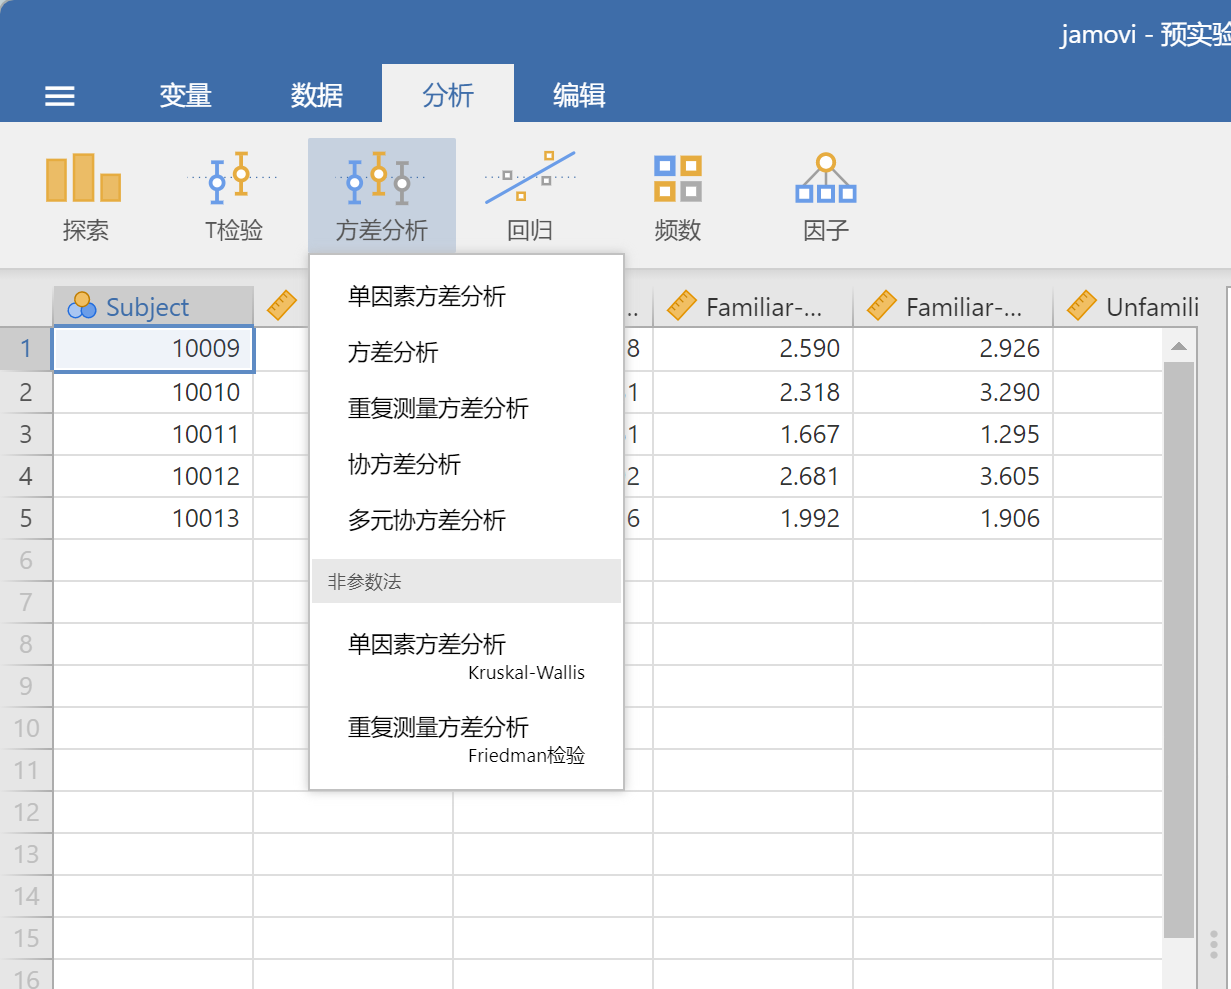
\includegraphics[width=0.8\linewidth]{img/jamovi/anova} 

}

\caption{方差分析}\label{fig:jamovi-anova}
\end{figure}

2.此次以重复测量方差分析为例。在下图左侧的界面里,左侧是我们数据的名称,右侧的``重复测量因子''是指在研究中设置的``被试内自变量''。在本例中,我们有三个``被试内自变量'',每个自变量都有两个水平。

\begin{figure}

{\centering 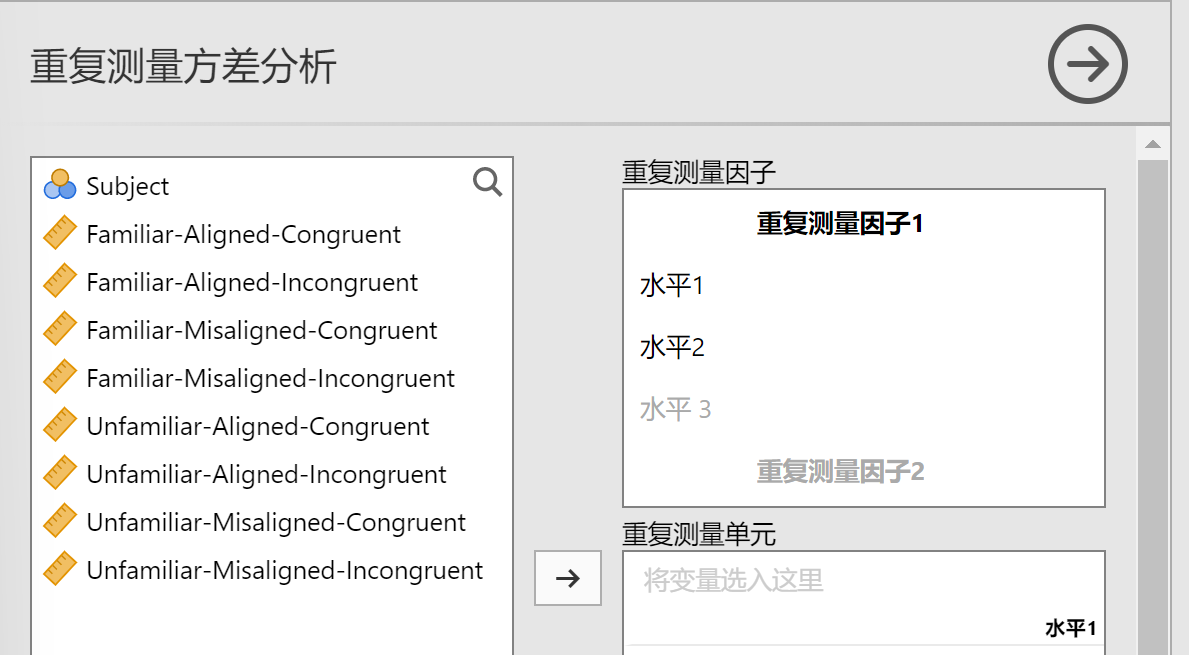
\includegraphics[width=0.6\linewidth]{img/jamovi/rmanova-factor} 

}

\caption{自变量}\label{fig:jamovi-rmanova-factor}
\end{figure}

3.例如我们将``重复测量因子1''定义为Familiar,它包括``familiar''和``unfamiliar''两个水平。

\begin{figure}

{\centering 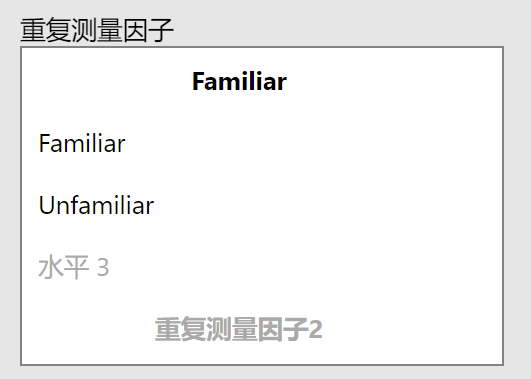
\includegraphics[width=0.4\linewidth]{img/jamovi/rmanova-factorlevels} 

}

\caption{自变量水平}\label{fig:jamovi-rmanova-factorlevels}
\end{figure}

4.定义好重复测量因子后,``重复测量单元''中会出现各个自变量水平的组合,而``重复测量单元''也就是指研究中的各种实验条件。在本例中我们的实验是一个2 * 2 * 2的被试内设计,所以共有8种实验条件,我们需要做的是将数据拖入其对应的重复测量单元中。

\begin{figure}

{\centering 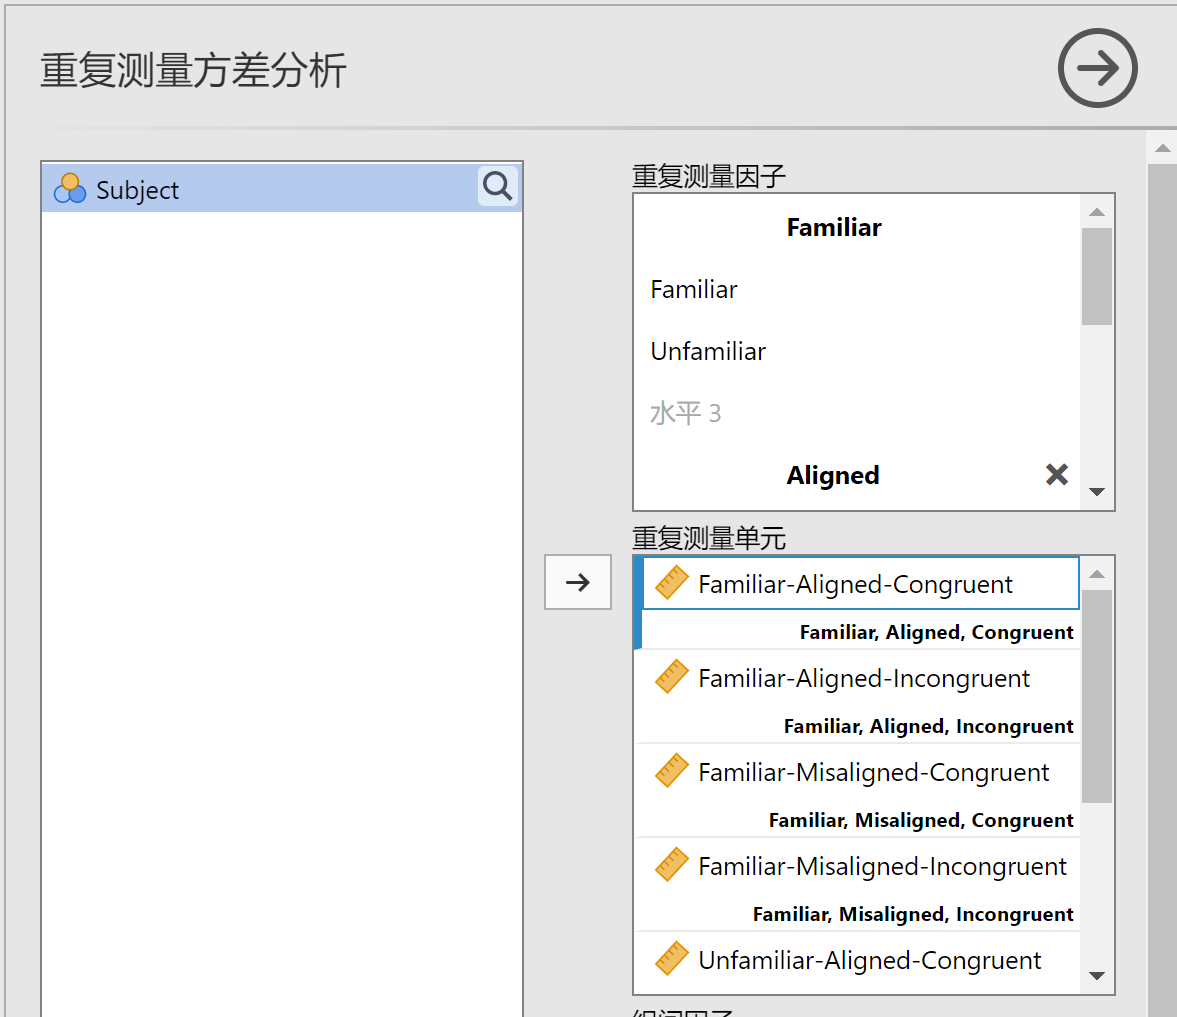
\includegraphics[width=0.6\linewidth]{img/jamovi/rmanova-factorlevels2} 

}

\caption{自变量水平2}\label{fig:jamovi-rmanova-factorlevels2}
\end{figure}

5.接下来我们要选择效应量为``偏η²值'',以及确定因变量标签。本例中因变量标签为``d-prime''.

\begin{figure}

{\centering 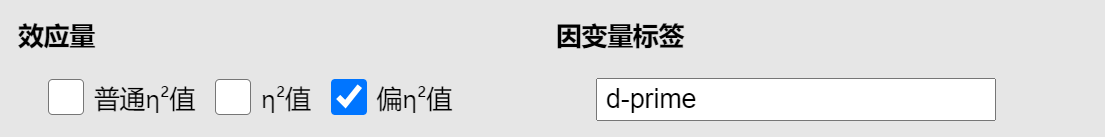
\includegraphics[width=0.6\linewidth]{img/jamovi/rmanova-dv} 

}

\caption{效应量偏η²}\label{fig:jamovi-rmanova-dv}
\end{figure}

6.下面的五个选项里,我们应当关注的主要是``适用条件判断''和``事后检验''。其中``事后检验''在之后的``2.2简单效应分析''一节中介绍。本节中我们先关注``适用条件判断''。

\begin{figure}

{\centering 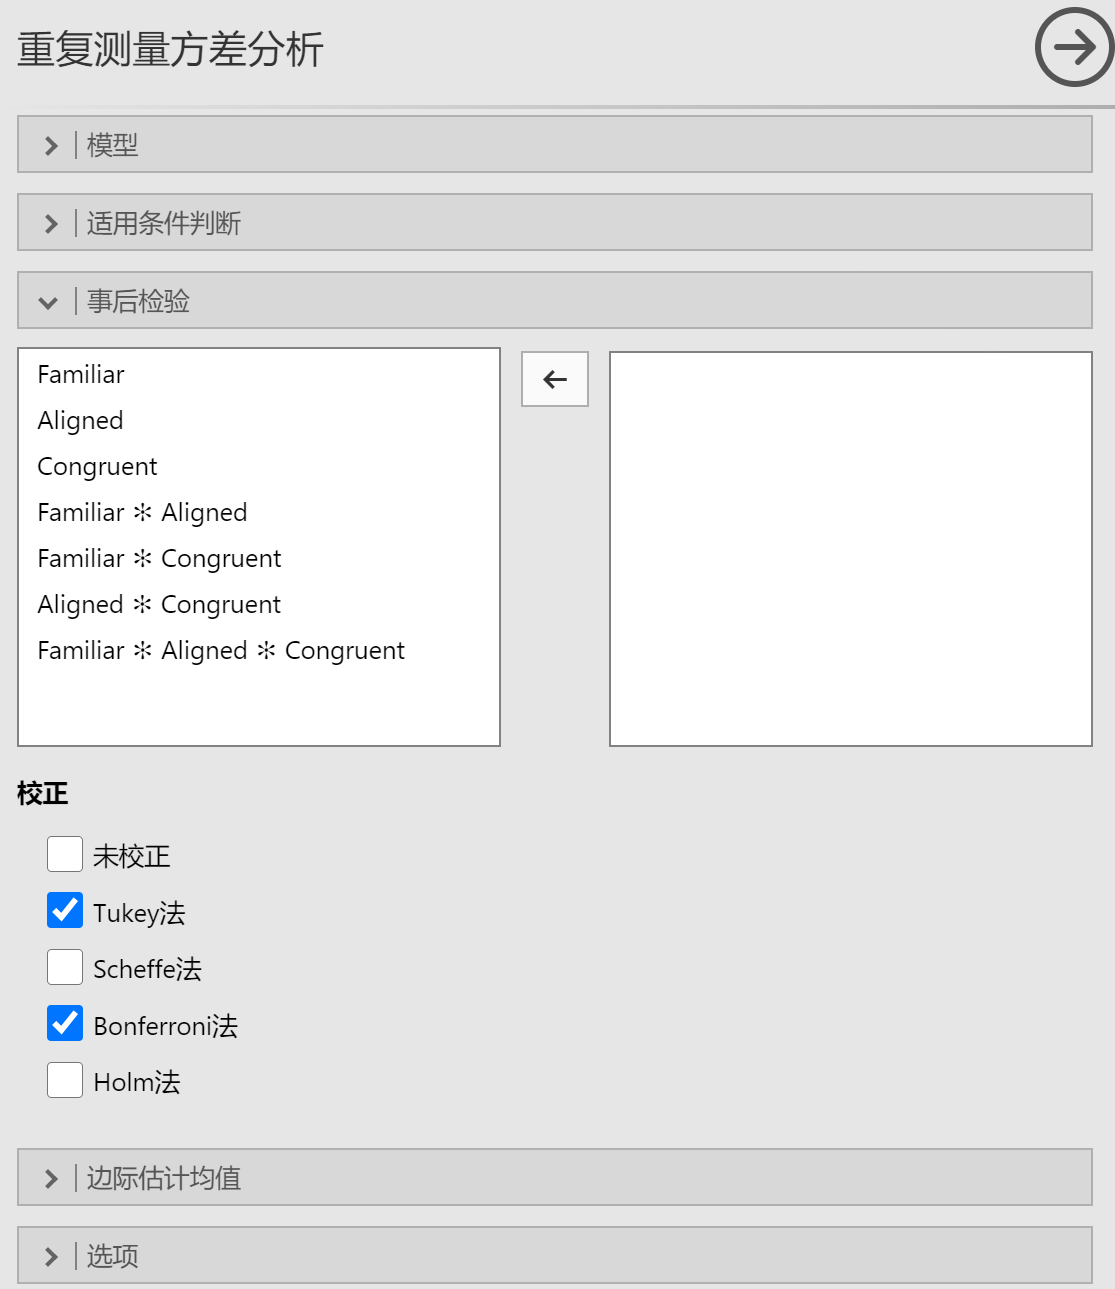
\includegraphics[width=0.6\linewidth]{img/jamovi/rmanova-posthoc} 

}

\caption{五个选项}\label{fig:jamovi-rmanova-posthoc1}
\end{figure}

7.对本专业来说,在``适用条件判断''这一栏中较为重要的是``方差齐性检验'',如果变量中涉及被试间变量,那么应当进行方差齐性检验。但由于本例中的变量都是被试内变量,所以无需进行方差齐性检验。其他几个选项也可以根据研究所需选取。

\begin{figure}

{\centering 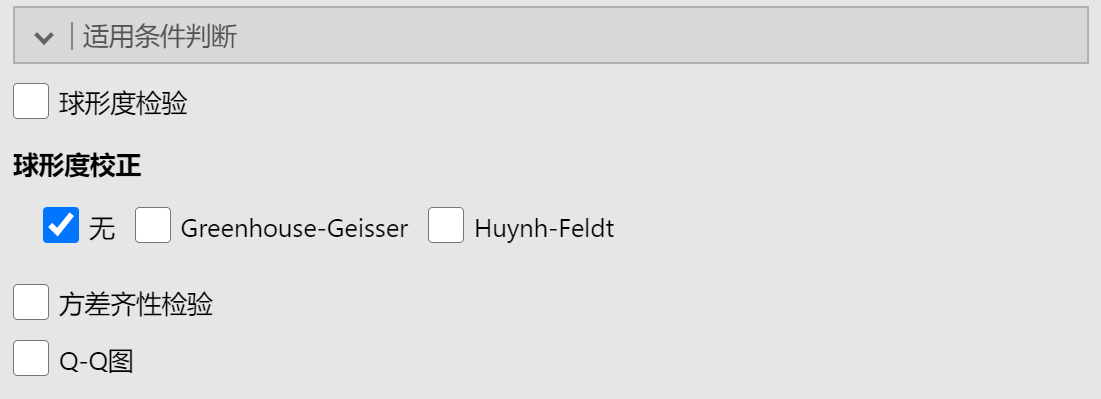
\includegraphics[width=0.6\linewidth]{img/jamovi/rmanova-sphericity} 

}

\caption{适用条件判断}\label{fig:jamovi-rmanova-sphericity}
\end{figure}

8.所有设定完成后,Jamovi会在右侧呈现数据分析结果。

\begin{figure}

{\centering 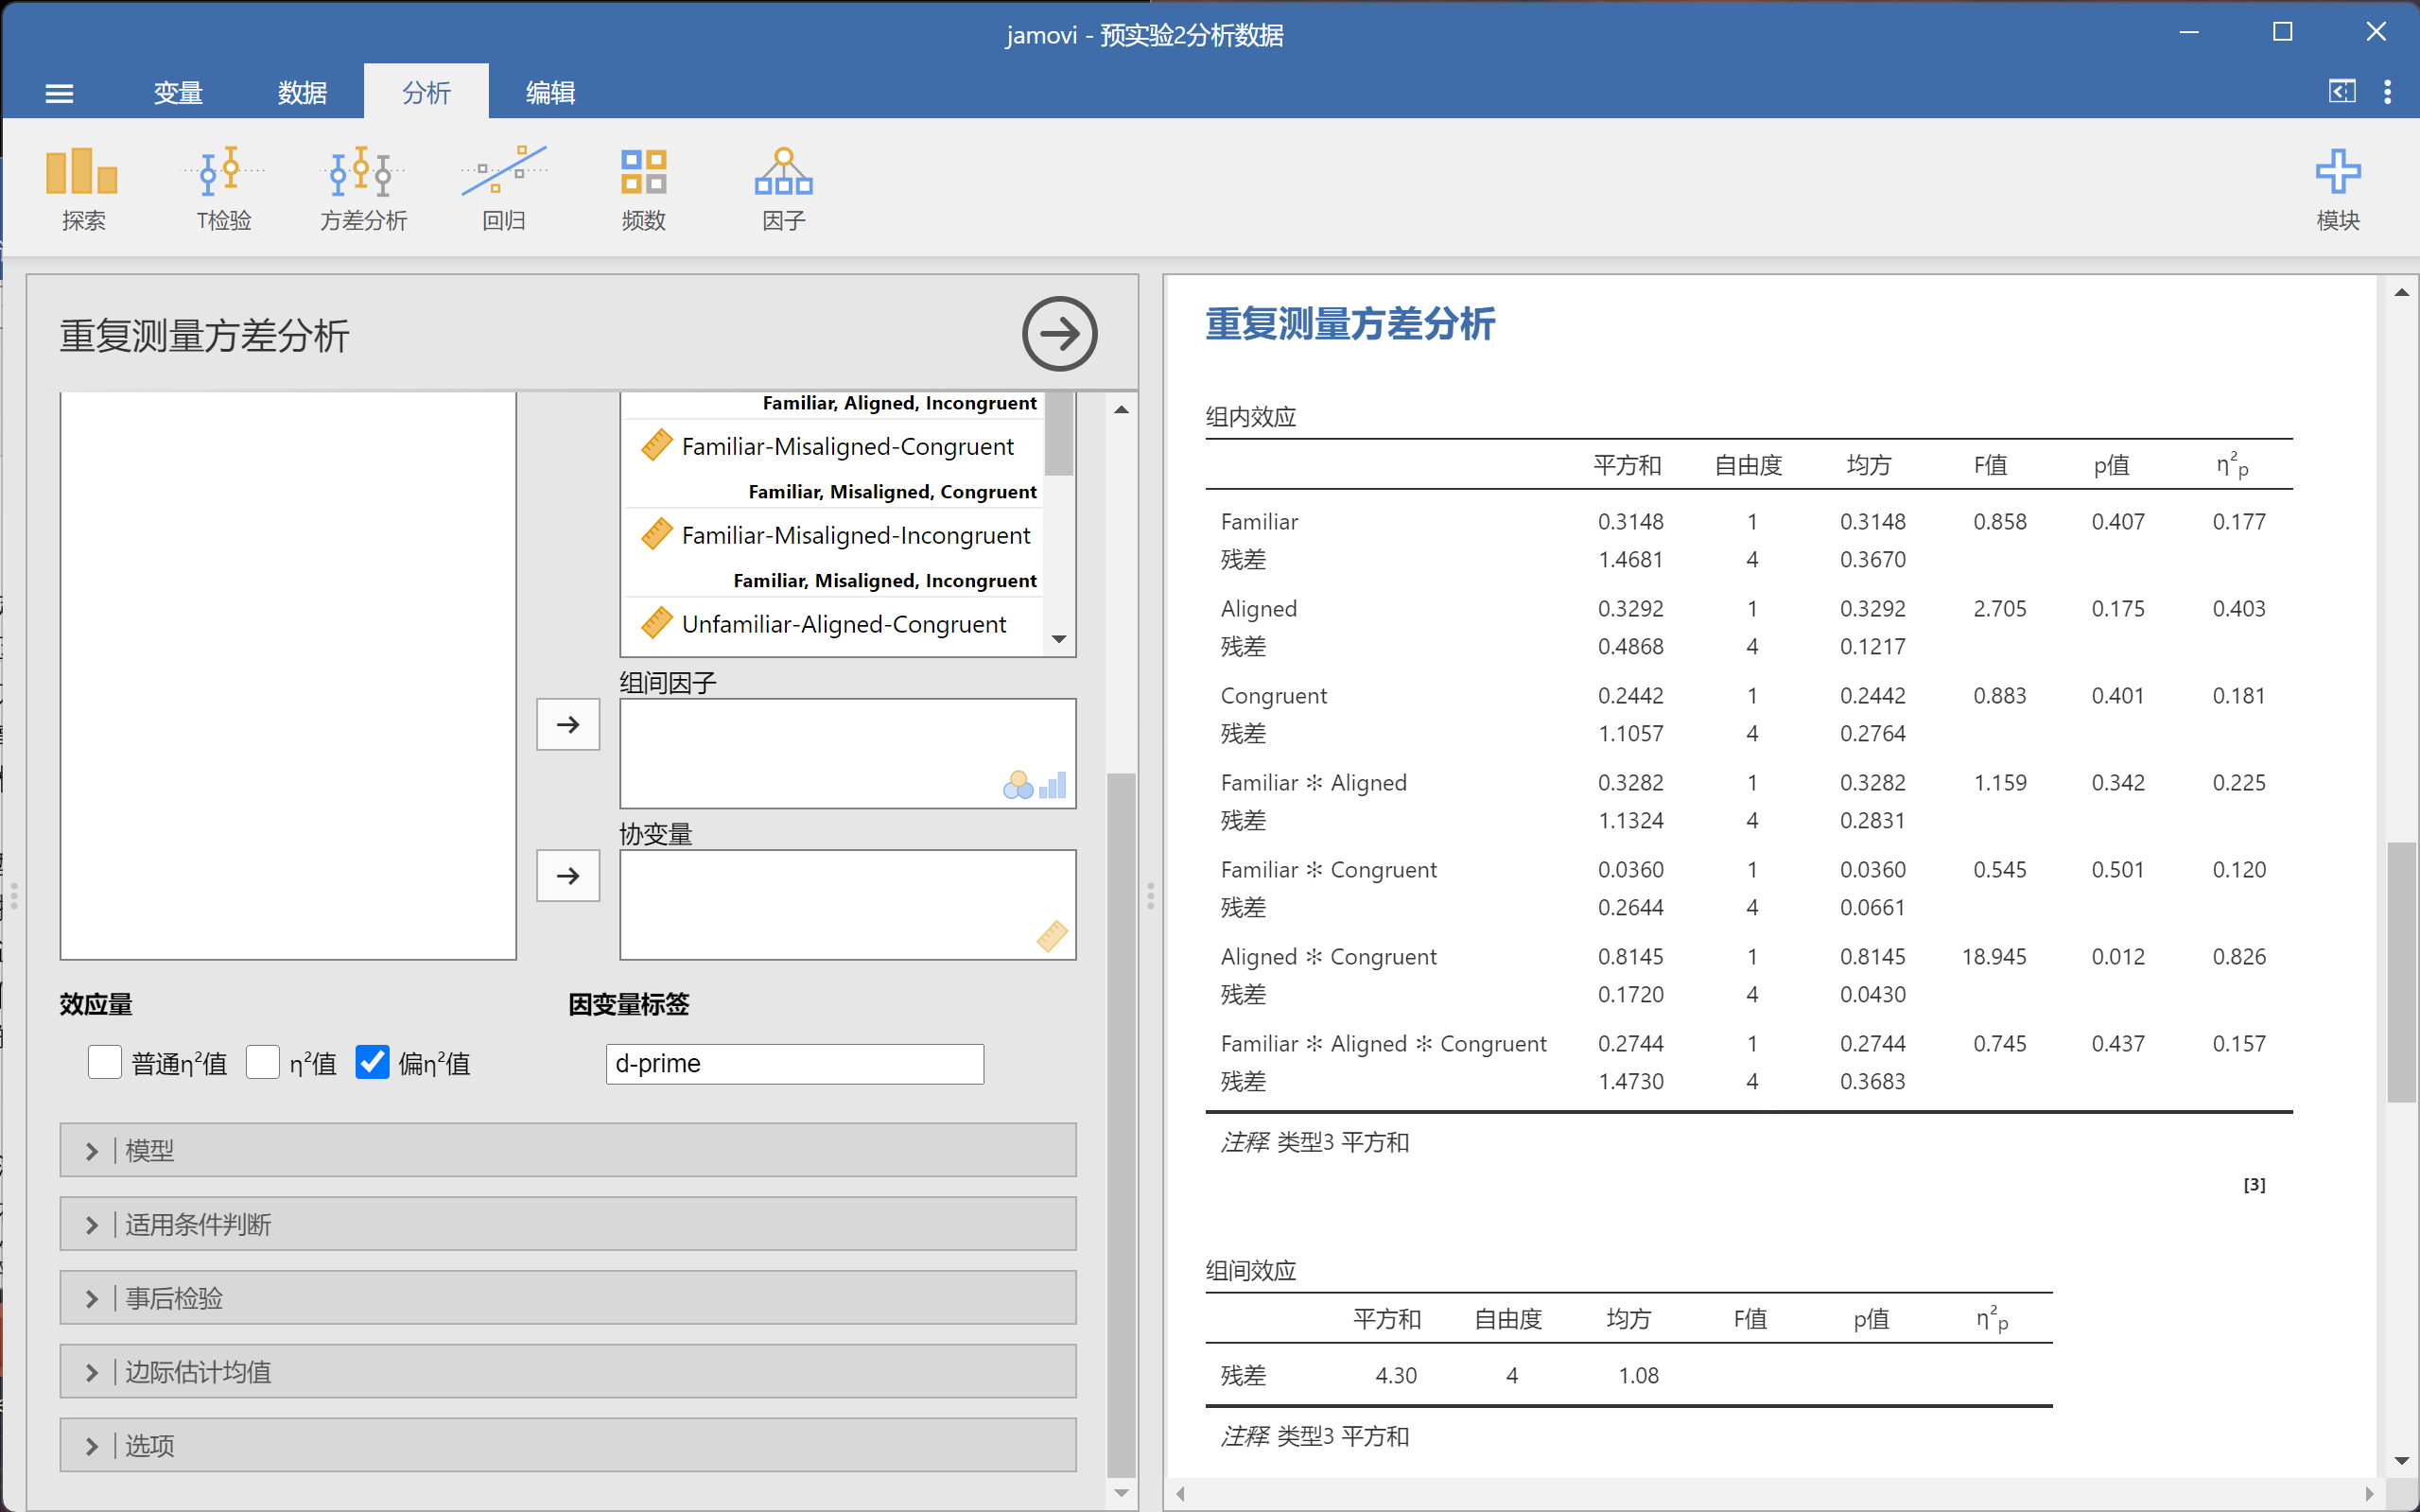
\includegraphics[width=1\linewidth]{img/jamovi/rmanova-result} 

}

\caption{方差分析结果}\label{fig:jamovi-rmanova-result}
\end{figure}

\section{简单效应分析}\label{ux7b80ux5355ux6548ux5e94ux5206ux6790}

如果F检验的结果表明差异不显著,说明实验中的自变量对因变量没有显著影响。相反,如果方差分析下检验的结果表明差异显著,拒绝了虚无假设,就表明几个实验处理组的两两比较中至少有一对平均数间的差异达到了显著水平,至于是哪一对,方差分析并没有回答。虚无假设被拒绝的结果一旦出现,就必须对各实验处理组的多对平均数进一步分析做深入比较,判断究竟是哪一对或哪几对的差异显著,哪几对不显著,确定两变量关系的本质,这就是事后检验(post hoc test)。这个统计分析过程也被称作事后多重比较(multiple comparison procedures)。

\subsection{重复测量方差分析中的简单效应分析}\label{ux91cdux590dux6d4bux91cfux65b9ux5deeux5206ux6790ux4e2dux7684ux7b80ux5355ux6548ux5e94ux5206ux6790}

这一部分承接上述重复测量方差分析。在本例中,当我们在Jamovi中确定好了``重复测量因子''即``被试内变量''和``重复测量单元''即``实验条件''后,我们可以看到右侧的结果栏中就可以呈现统计结果,如果某两个或几个变量之间存在显著的交互作用,那么我们应当进行事后检验,以确定一个变量在与它有交互作用的另一个变量的哪些水平上显著,哪些水平上不显著。

1.我们需要先选择下列五个选项中的``事后检验''。再选择需要进行事后检验的交互变量,并按照研究需要选择恰当的校正方法。

\begin{figure}

{\centering 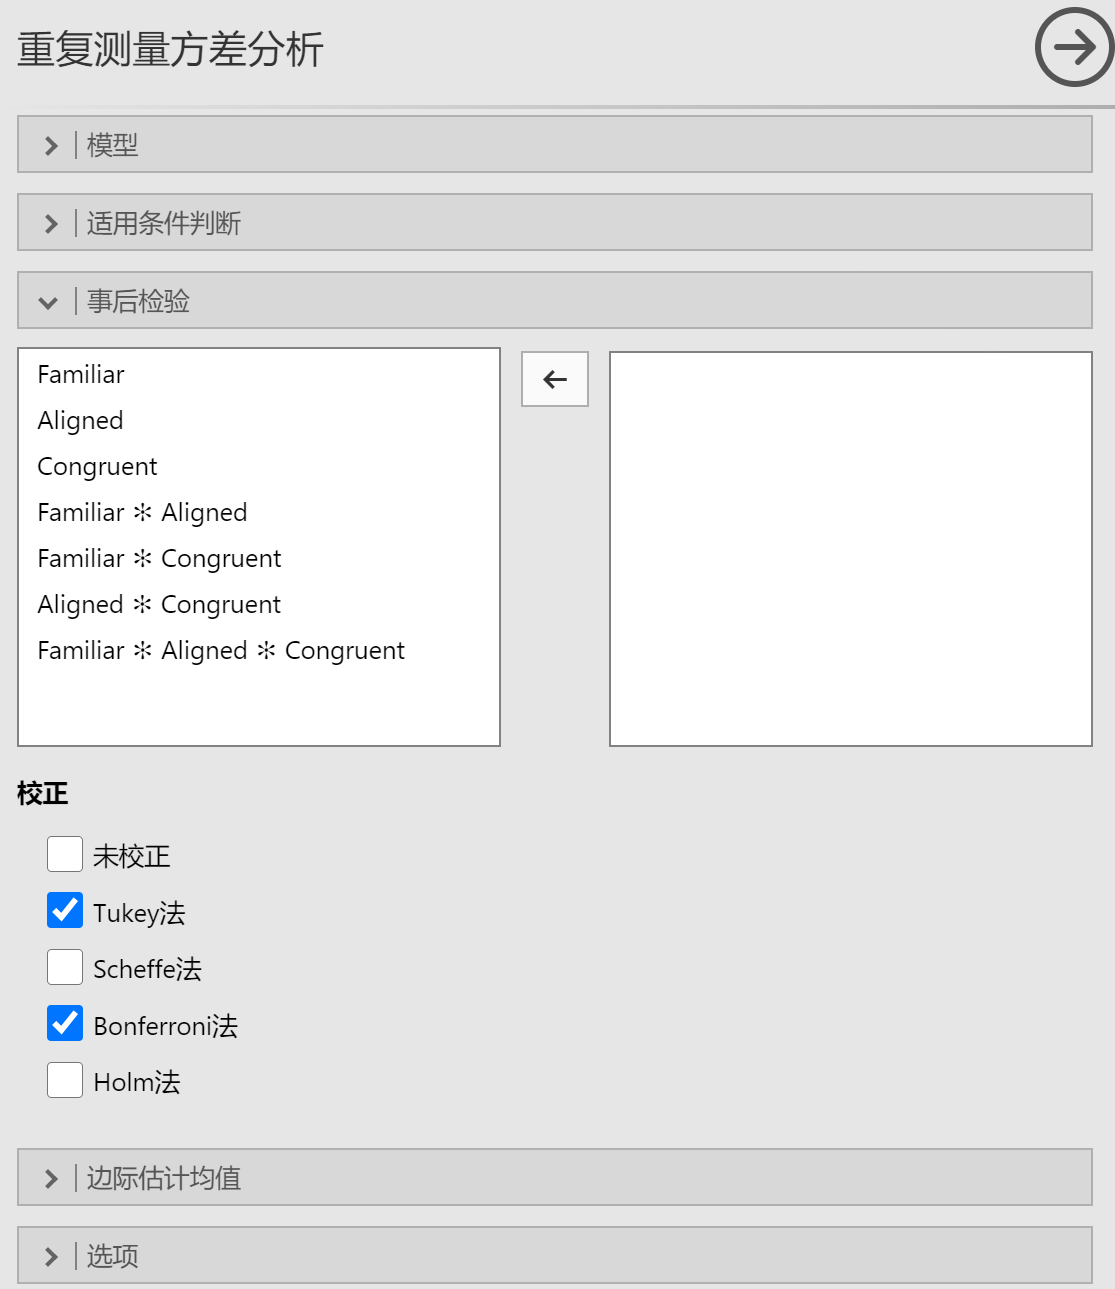
\includegraphics[width=0.6\linewidth]{img/jamovi/rmanova-posthoc} 

}

\caption{事后检验}\label{fig:jamovi-rmanova-posthoc2}
\end{figure}

2.右侧窗口会生成事后检验的结果,其中最右边两列就是Jamovi按照我们选择的``Tukey法''和``Bonferron法''计算出的统计量。

\begin{figure}

{\centering 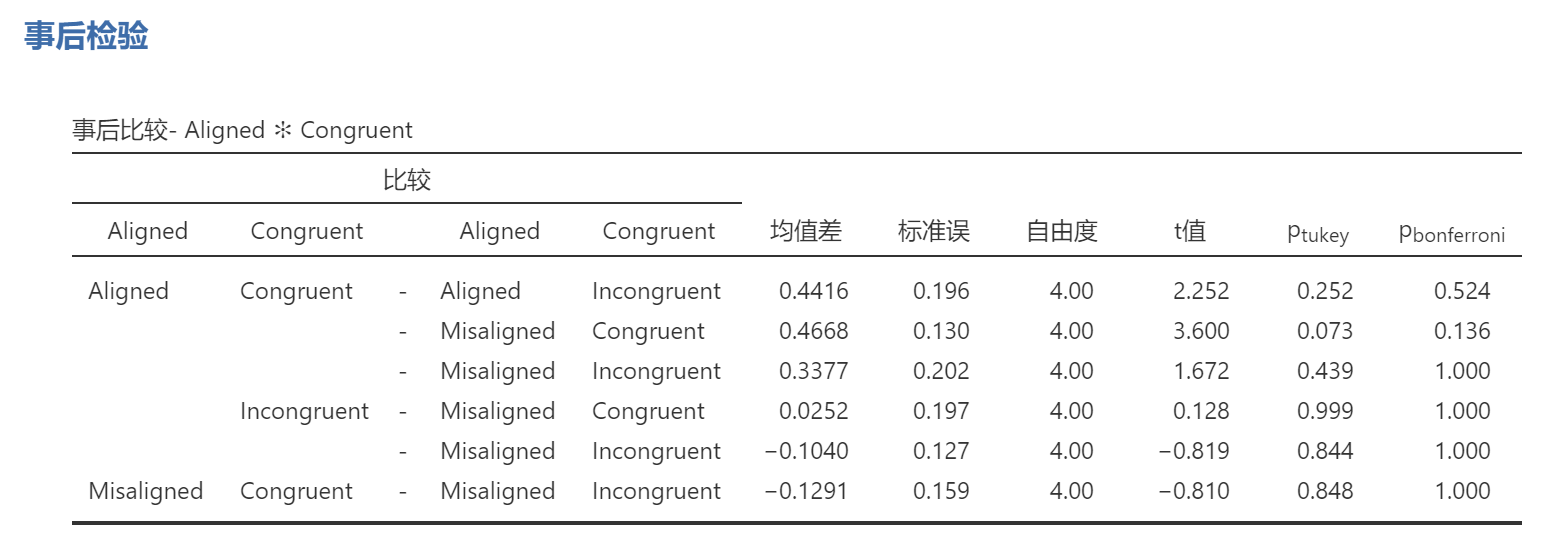
\includegraphics[width=1\linewidth]{img/jamovi/rmanova-posthoc-results} 

}

\caption{事后检验结果}\label{fig:jamovi-rmanova-posthoc-results}
\end{figure}

\section{T检验}\label{tux68c0ux9a8c}

\begin{itemize}
\tightlist
\item
  首先,导入数据
\item
  其次,点击选项栏的分析,选择对应的T检验。
\end{itemize}

\begin{figure}

{\centering 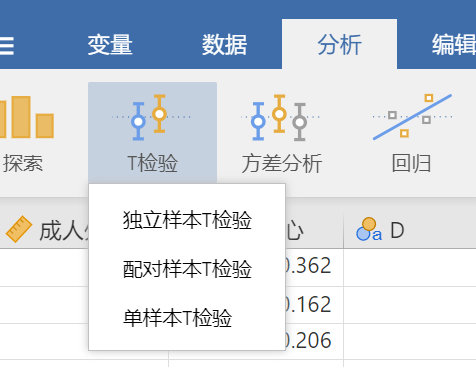
\includegraphics[width=0.5\linewidth]{img/jamovi/ttest} 

}

\caption{T检验}\label{fig:jamovi-ttest}
\end{figure}

\subsection{配对样本T检验}\label{ux914dux5bf9ux6837ux672ctux68c0ux9a8c}

本例中介绍``配对样本T检验''。接着,选择要分析的变量

\begin{figure}

{\centering 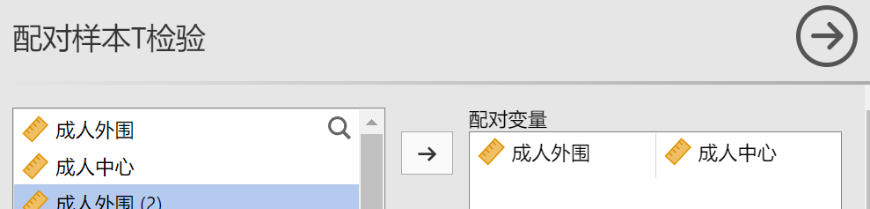
\includegraphics[width=0.6\linewidth]{img/jamovi/ttest-compare} 

}

\caption{变量选择}\label{fig:jamovi-ttest-compare}
\end{figure}

\begin{itemize}
\tightlist
\item
  然后,可以按需勾选,描述就是分析数据的均值、标准差、标准误等描述性数据;描述图就是生成图表
\end{itemize}

\begin{figure}

{\centering 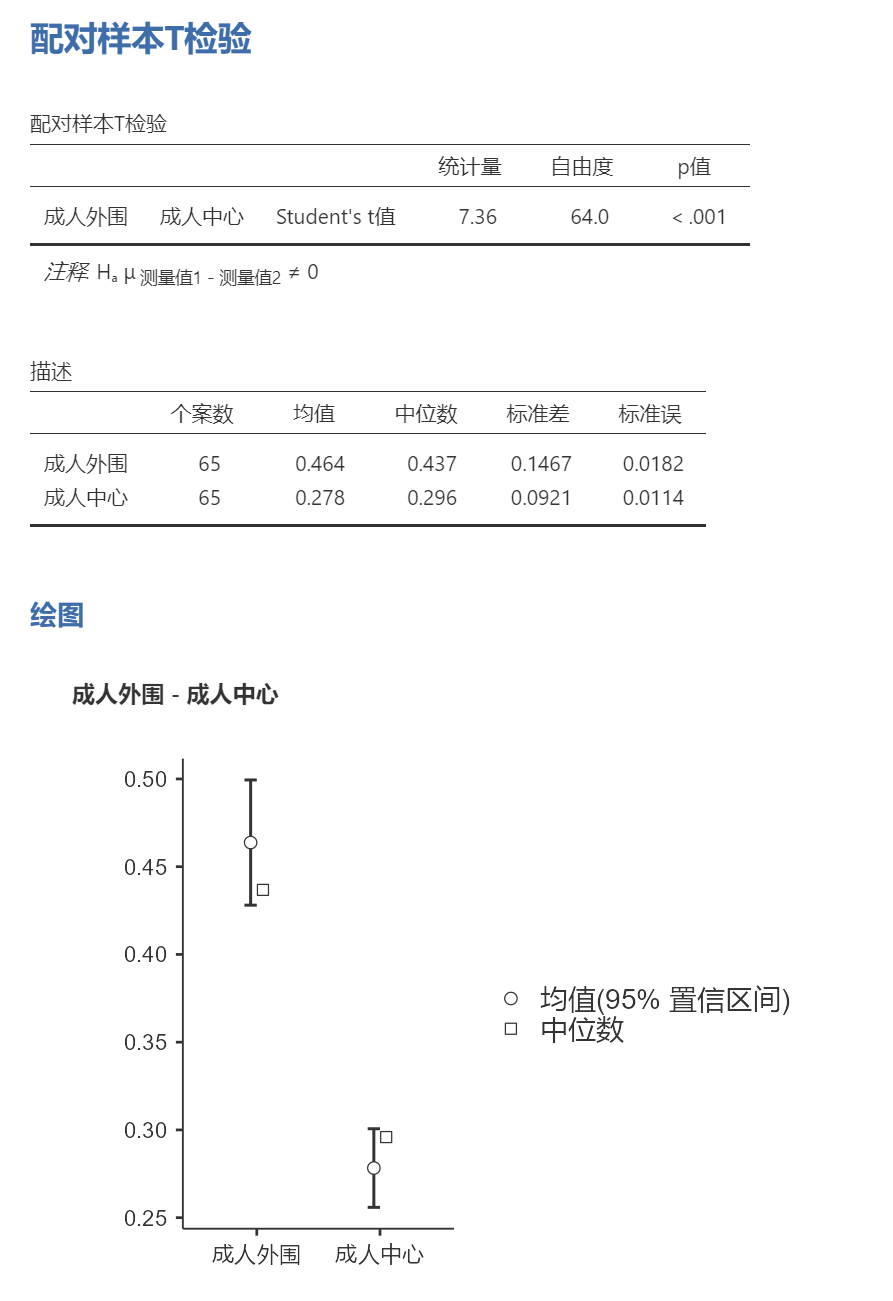
\includegraphics[width=0.8\linewidth]{img/jamovi/ttest-results} 

}

\caption{配对样本T检验结果}\label{fig:jamovi-ttest-results}
\end{figure}

\section{额外模块推荐}\label{ux989dux5916ux6a21ux5757ux63a8ux8350}

\begin{figure}

{\centering 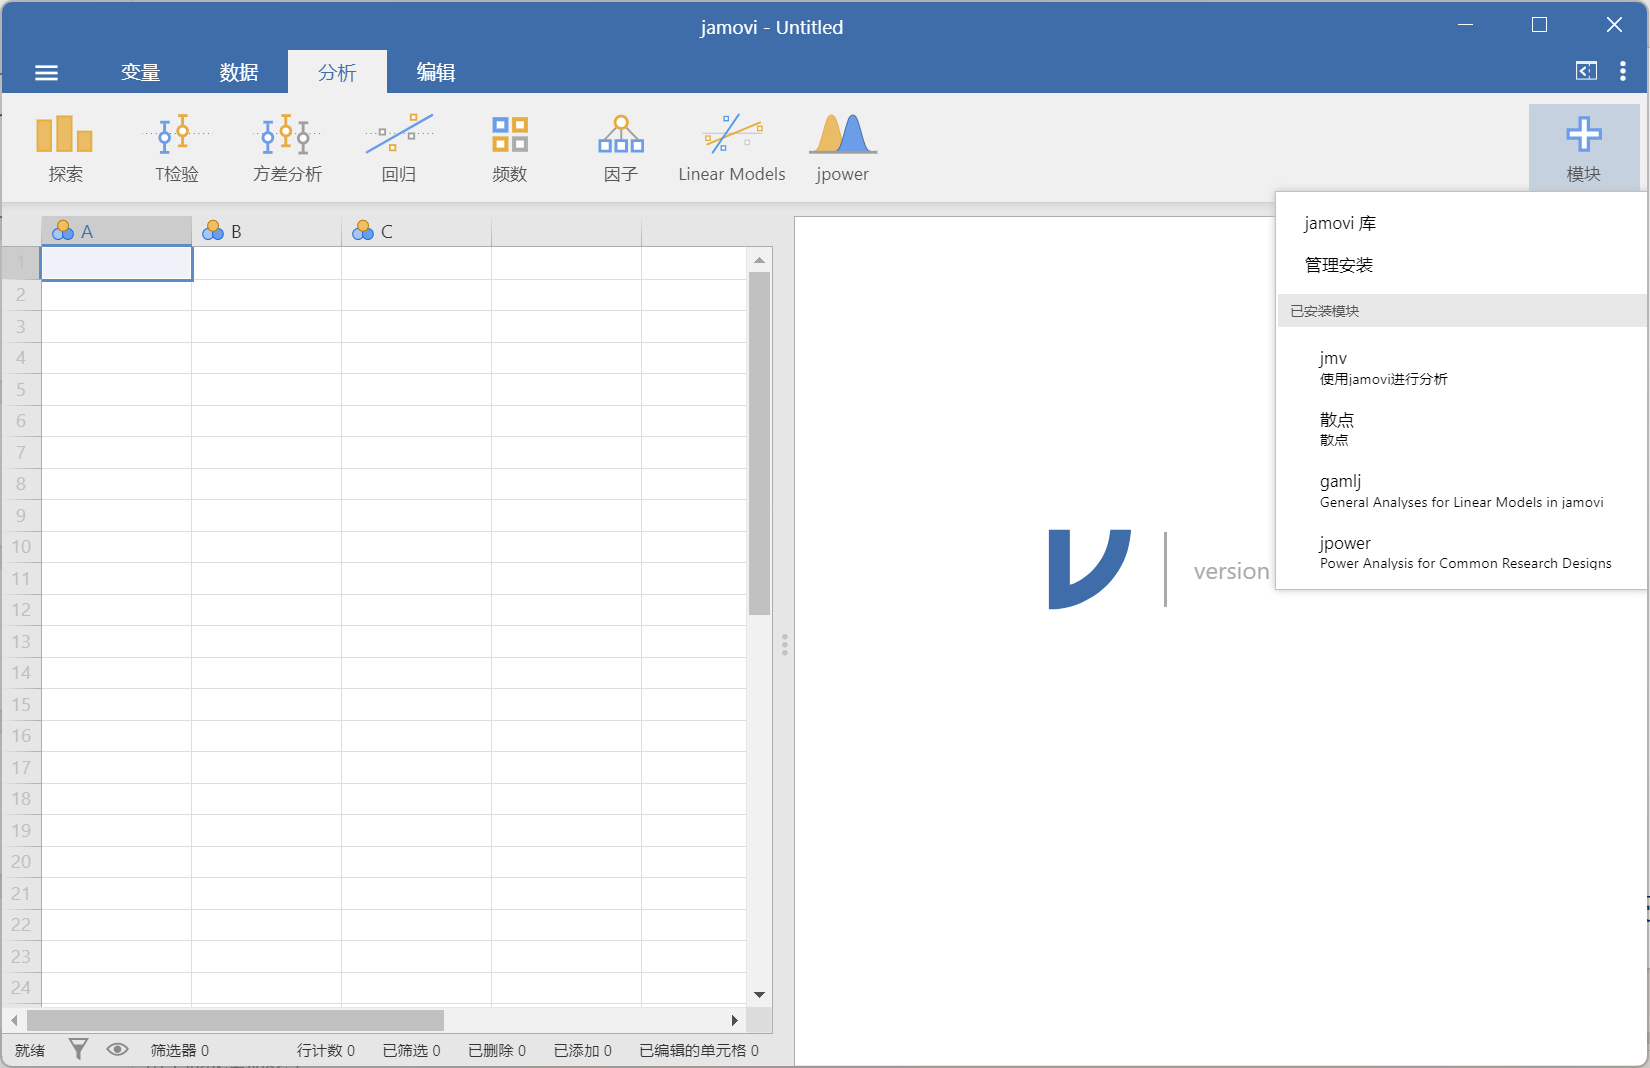
\includegraphics[width=1\linewidth]{img/jamovi/modules} 

}

\caption{添加额外模块}\label{fig:jamovi-modules}
\end{figure}

\begin{figure}

{\centering 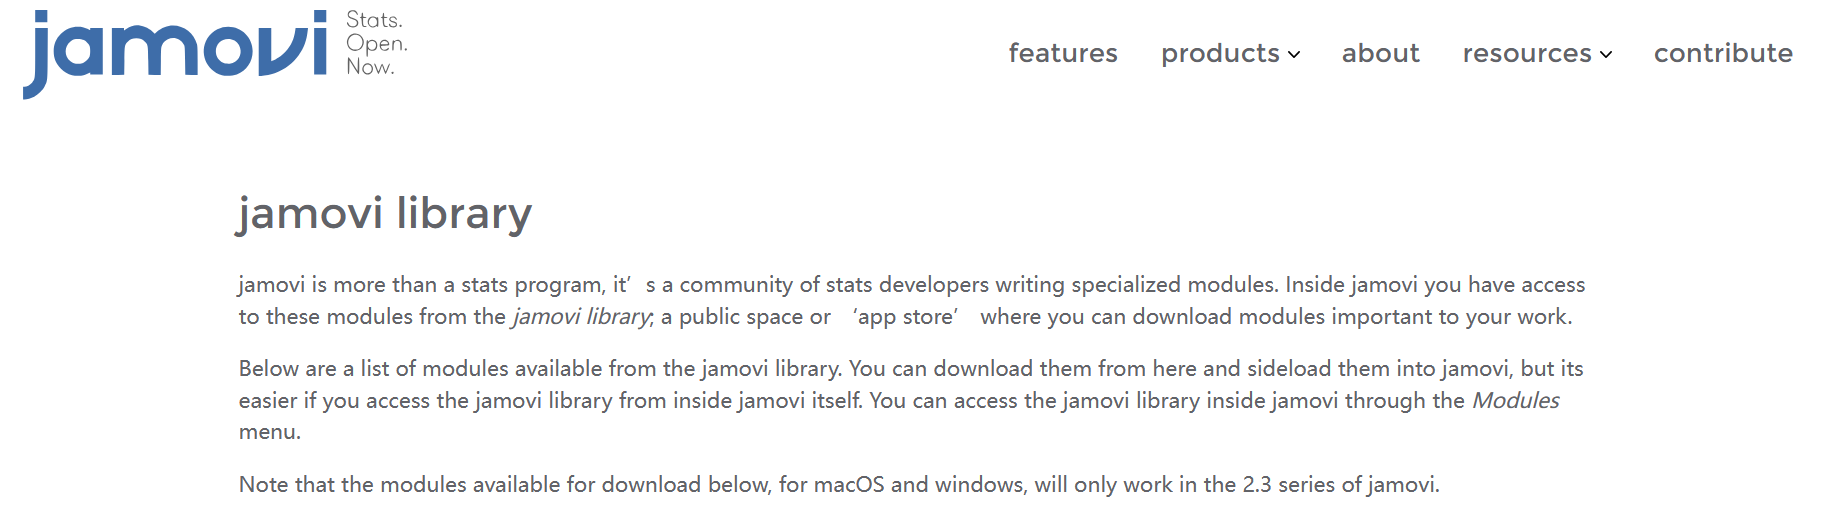
\includegraphics[width=1\linewidth]{img/jamovi/modules-library} 

}

\caption{额外模块库}\label{fig:jamovi-modules-library}
\end{figure}

可以通过jamovi官网下载自己所需要的库。这是网址:\url{https://www.jamovi.org/library.html}

\begin{figure}

{\centering 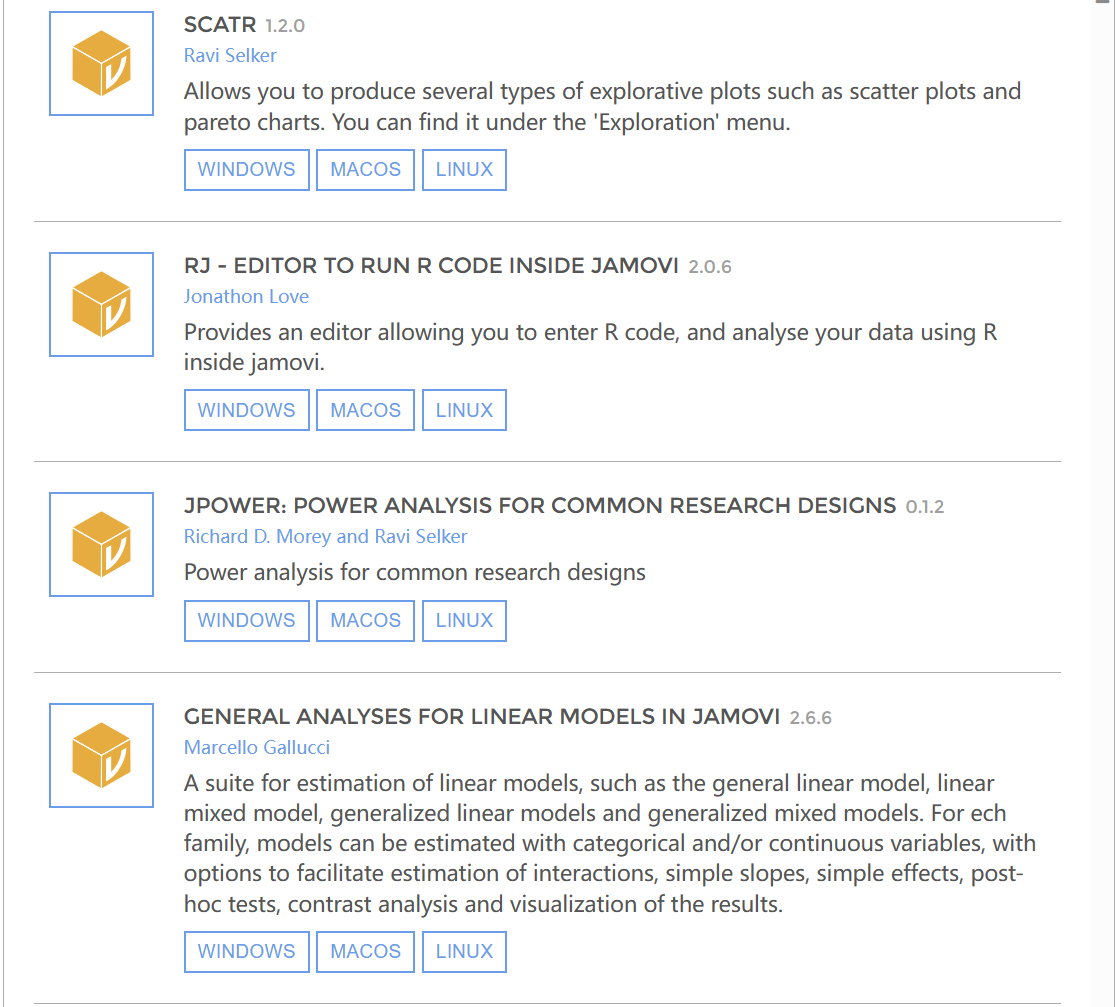
\includegraphics[width=1\linewidth]{img/jamovi/modules1} 

}

\caption{额外模块}\label{fig:jamovi-modules1}
\end{figure}

\begin{figure}

{\centering 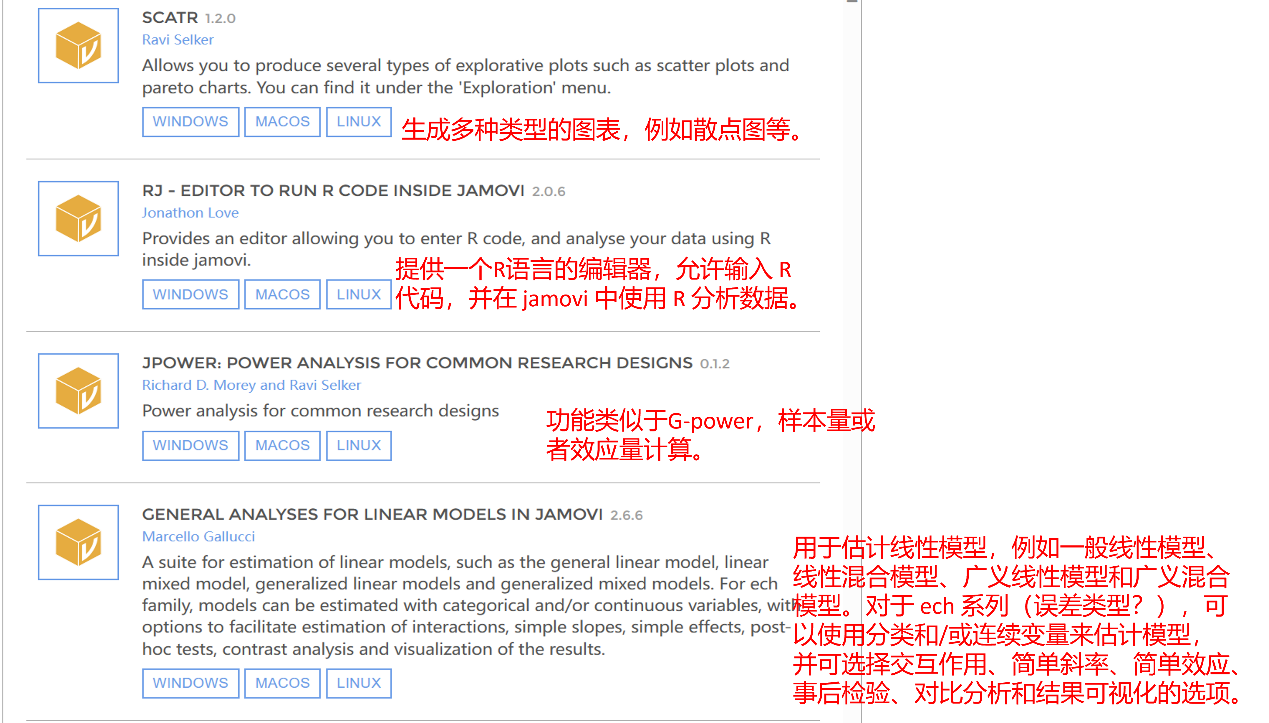
\includegraphics[width=1\linewidth]{img/jamovi/modules2} 

}

\caption{额外模块1}\label{fig:jamovi-modules2}
\end{figure}

\begin{figure}

{\centering 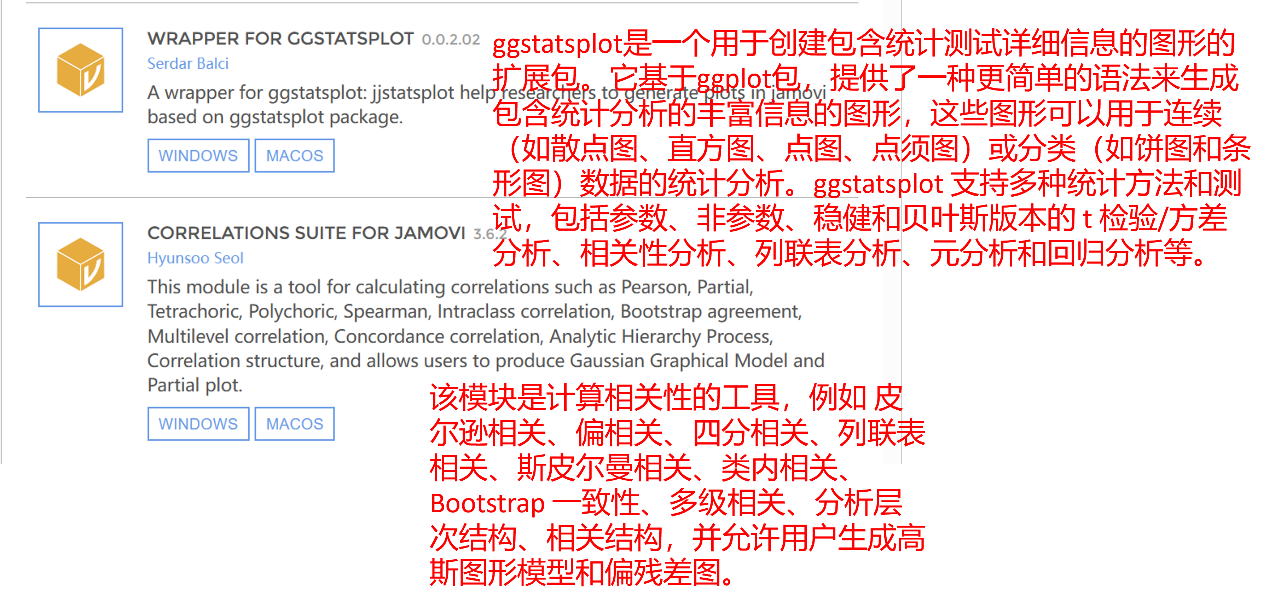
\includegraphics[width=1\linewidth]{img/jamovi/modules3} 

}

\caption{额外模块2}\label{fig:jamovi-modules3}
\end{figure}

\begin{figure}

{\centering 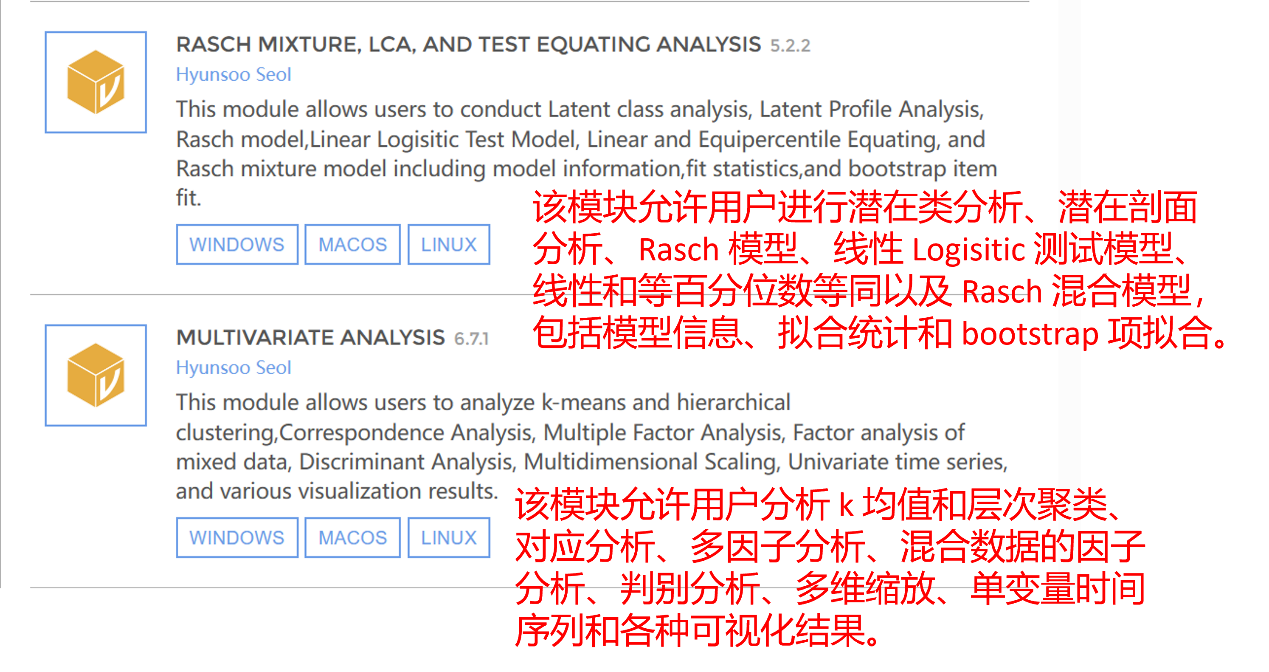
\includegraphics[width=1\linewidth]{img/jamovi/modules4} 

}

\caption{额外模块3}\label{fig:jamovi-modules4}
\end{figure}

\chapter{R语言}\label{r}

\section{预处理数据}\label{r-prepro}

汇总:
更新于:

\section{重复测量方差分析}\label{r-rm-anova}

汇总:
更新于:

\section{数据可视化}\label{r-plot}

汇总:
更新于:

\section{RStudio Shortcut Keys}\label{RStudioShortcutKeys}

汇总:郭沫然\\
更新于:2024-12-16

\begin{longtable}[]{@{}lll@{}}
\toprule\noalign{}
Console & & \\
\midrule\noalign{}
\endhead
\bottomrule\noalign{}
\endlastfoot
\textbf{Description} & \textbf{Windows} & \textbf{Mac} \\
将光标定位到控制台 & Ctrl+2 & Ctrl+2 \\
在历史命令中导航 & Up/Down & Up/Down \\
\textbf{Source} & & \\
\textbf{Description} & \textbf{Windows} & \textbf{Mac} \\
保存当前文件 & Ctrl+S & Command+S \\
插入块 & Ctrl+Alt+I & Command+Option+I \\
运行当前/被选中的代码 & Ctrl+Enter & Command+Enter \\
再次运行以前区域 & Ctrl+Shift+P & Command+Shift+P \\
运行当前文件 & Ctrl+Alt+R & Command+Option+R \\
运行当前函数定义代码 & Ctrl+Alt+F & Command+Option+F \\
运行当前代码块 & Ctrl+Alt+C & Command+Option+C \\
运行下一个代码块 & Ctrl+Alt+N & Command+Option+N \\
执行一个外部文件中的代码 & Ctrl+Shift+O & Command+Shift+O \\
切换tab & Ctrl+Alt+Down & Ctrl+Option+Down \\
Reindent lines & Ctrl+I & Command+I \\
注释/取消注释 当前行/选中区域 & Ctrl+Shift+C & Command+Shift+C \\
Reflow comment & Ctrl+Shift+/ & Command+Shift+/ \\
Transpose Letters & Ctrl+T & \\
查找并替换 & Ctrl+F & Command+F \\
查找下一个 & Win: F3, Linux: Ctrl+G & Command+G \\
查找上一个 & Win: Shift+F3, & Command+Shift+G \\
替换并查找 & Ctrl+= & Command+= \\
\textbf{Editing (Console and Source)} & & \\
\textbf{Description} & \textbf{Windows} & \textbf{Mac} \\
撤销 & Ctrl+Z & Command+Z \\
重复上次撤销的操作 & Ctrl+Shift+Z & Command+Shift+Z \\
剪切 & Ctrl+X & Command+X \\
复制 & Ctrl+C & Command+C \\
粘贴 & Ctrl+V & Command+V \\
全选 & Ctrl+A & Command+A \\
删除行 & Ctrl+D & Command+D \\
选择 & Shift+{[}Arrow{]} & Shift+{[}Arrow{]} \\
选择一个词 & Ctrl+Shift+Left/Right & Option+Shift+Left/Right \\
缩进 & Tab (at beginning of line) & \\
取消缩进 & Shift+Tab & Shift+Tab \\
查看光标处的函数帮助 & F1 & F1 \\
自动完成 & Tab or Ctrl+Space & Tab or Command+Space \\
\end{longtable}

\part{科研工具}\label{part-ux79d1ux7814ux5de5ux5177}

\chapter{Zotero}\label{zotero}

汇总:郭沫然\\
更新于:2025-01-06

\section{下载安装}\label{ux4e0bux8f7dux5b89ux88c5}

\href{https://www.zotero.org/}{官方下载网址}

可以直接参考下方链接网址里的安装教程进行安装配置。

\href{https://blog.csdn.net/qq_47885795/article/details/141631652?spm=1001.2014.3001.5506}{zotero安装教程}

其中的第二部分 ``配置'' 有需要可以参考但并非日常使用所必要的。可以只看 ``安装'' 部分以及后面的 ``安装插件'' 部分。

\section{功能简介}\label{ux529fux80fdux7b80ux4ecb}

\subsection{zotero是做什么的}\label{zoteroux662fux505aux4ec0ux4e48ux7684}

Zotero是一个参考文献管理器。用来存储、管理和引用参考文献,比如书籍、文章和期刊等。在Zotero中,将每一个文献作为一个条目储存,每一个条目当中可以包含与之相关的其他多种信息和附加条目。

广泛地说,Zotero是收集和组织研究信息和资源的工具。
可以储存并管理的条目类型广泛,几乎可以是任何东西,包括书籍、文章、报告、网页、艺术品、电影、信件、手稿、录音、账单、案例或法规等等。

\begin{figure}

{\centering 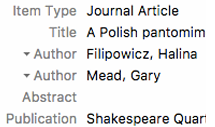
\includegraphics[width=0.4\linewidth]{img/zotero/zotero_workInform} 

}

\caption{作品信息}\label{fig:zotero-workInform}
\end{figure}

\begin{figure}

{\centering 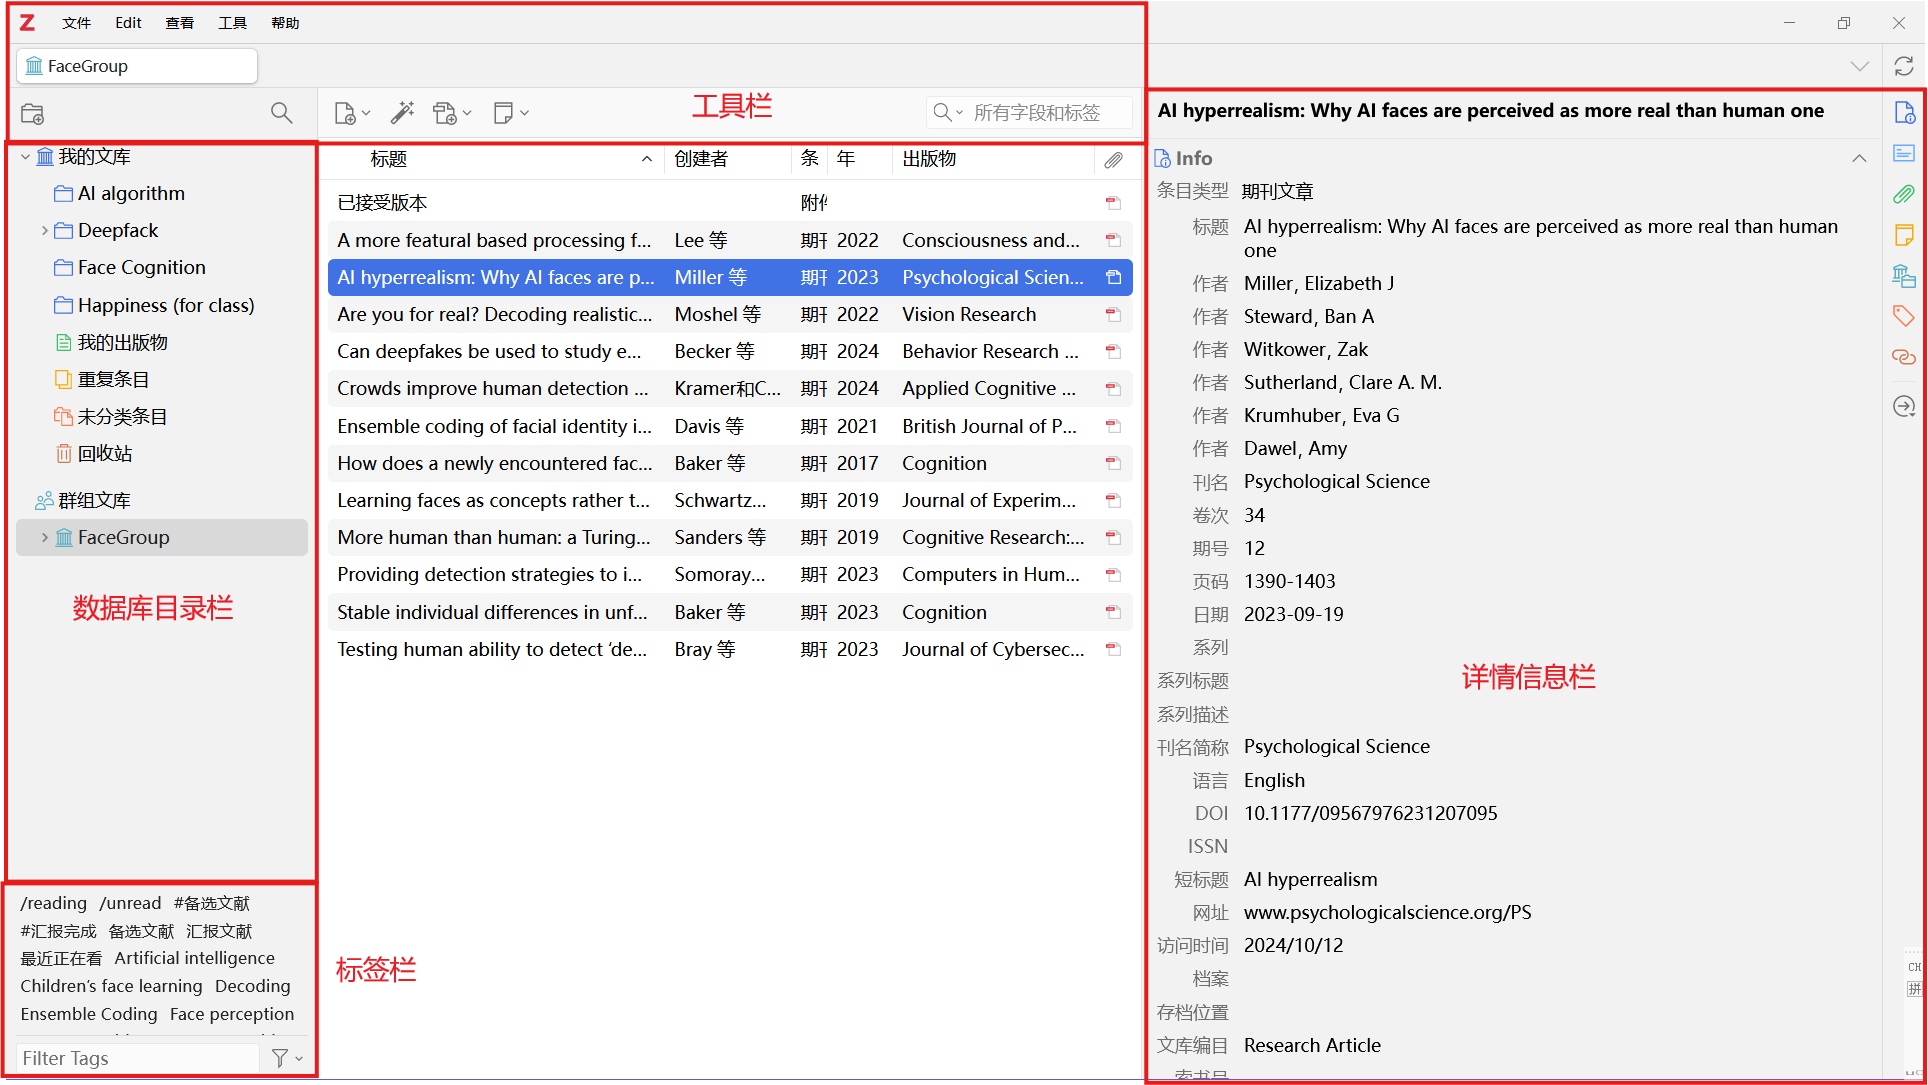
\includegraphics[width=1\linewidth]{img/zotero/zotero_interface} 

}

\caption{主界面}\label{fig:zotero-interface}
\end{figure}

通常储存的条目显示在Zotero的中心列表中。条目的相关信息显示在右列表中。包括标题、创建者、出版商、日期、页码以及引用条目所需的任何其他数据。

\begin{figure}

{\centering 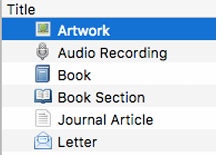
\includegraphics[width=0.4\linewidth]{img/zotero/zotero_worktype} 

}

\caption{作品类型}\label{fig:zotero-worktype}
\end{figure}

\subsection{用于管理条目的功能}\label{ux7528ux4e8eux7ba1ux7406ux6761ux76eeux7684ux529fux80fd}

\subsubsection{文件夹:}\label{ux6587ux4ef6ux5939}

右键单击``我的图书馆''或单击左侧窗格上方的``新收藏''按钮,以创建一个文件夹,可以用来分类存放文献条目。同一个条目可以同时属于多个收藏夹。

\begin{figure}

{\centering 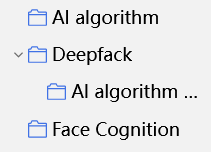
\includegraphics[width=0.4\linewidth]{img/zotero/zotero_list} 

}

\caption{文件夹列表}\label{fig:zotero-list}
\end{figure}

\subsubsection{标签:}\label{ux6807ux7b7e}

标签是自己命名的。可以对每一个条目根据需要分配多少个标签。使用左侧列表底部的标签选择器或通过右侧信息列表中的标签选项卡添加或删除标签。标签的颜色一共有六个。在阅读文献的过程中不断地为文献添加标签,可以更好管理文献,配合上搜索功能,可以提高对于文献的管理效率。

\begin{figure}

{\centering 
\includegraphics[width=0.9\linewidth]{img/zotero/zotero_tag} 

}

\caption{标签}\label{fig:zotero-tag}
\end{figure}

\subsubsection{搜索功能以及对搜索的储存:}\label{ux641cux7d22ux529fux80fdux4ee5ux53caux5bf9ux641cux7d22ux7684ux50a8ux5b58}

Zotero支持对条目进行快速搜索,包括储存条目的信息数据,标签,或全文内容匹配搜索等,在Zotero工具栏中找到搜索选项。点击搜索框图标会打开高级搜索列表,允许进行更复杂或更窄范围的搜索。另外高级搜索结果可以保存在左侧条目列表中,类似于一个集合,会自动更新新的匹配条目。

\begin{figure}

{\centering 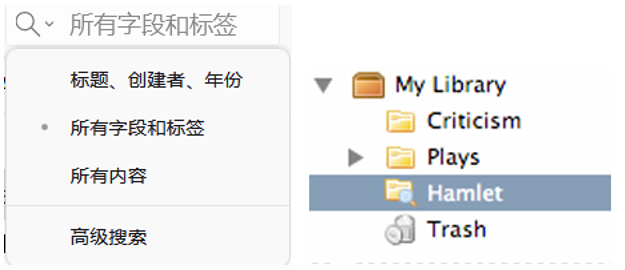
\includegraphics[width=0.8\linewidth]{img/zotero/zotero_search} 

}

\caption{搜索}\label{fig:zotero-search}
\end{figure}

\subsection{储存条目及其附件}\label{ux50a8ux5b58ux6761ux76eeux53caux5176ux9644ux4ef6}

\subsubsection{附件及其类型:}\label{ux9644ux4ef6ux53caux5176ux7c7bux578b}

条目可以附加注释、文件和链接等附件。这些附件会列在条目下方的列表中。通过点击条目旁边的箭头可以显示或隐藏附件。任何类型的文件都可以附加到条目中。使用Zotero工具栏中的``添加附件(回形针)''按钮,通过右键点击条目或者通过拖放来添加附件。当在浏览器中使用Zotero连接器导入条目时,也可以自动下载相关文件,如文献的PDF原文或是相关网页等。

\begin{figure}

{\centering 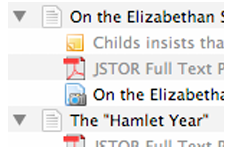
\includegraphics[width=0.4\linewidth]{img/zotero/zotero_attachment} 

}

\caption{附件}\label{fig:zotero-attachment}
\end{figure}

\subsubsection{从浏览器行直接导入条目:}\label{ux4eceux6d4fux89c8ux5668ux884cux76f4ux63a5ux5bfcux5165ux6761ux76ee}

使用Chrome、Firefox或Edge的Zotero连接器,可以很轻松地从网页上将文献导入Zotero中从而创建新的储存条目。只需点击连接器按钮,Zotero就可以自动创建适当类型的条目并识别和填充条目的相关信息字段。

\begin{figure}

{\centering 
\includegraphics[width=0.9\linewidth]{img/zotero/zotero_connector} 

}

\caption{浏览器连接器}\label{fig:zotero-connector}
\end{figure}

\subsubsection{网页保存:}\label{ux7f51ux9875ux4fddux5b58}

如果Zotero连接器不能识别页面上的数据,它仍然可以将文献的页面保存为带有网页快照附加的储存网页的条目。虽然这样会保存基本的信息数据(标题、URL、访问日期等),但还是需要手动填写额外的信息以及附件。

\begin{figure}

{\centering 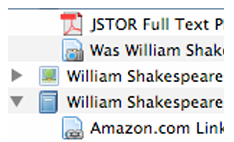
\includegraphics[width=0.4\linewidth]{img/zotero/zotero_websave} 

}

\caption{网页快照}\label{fig:zotero-websave}
\end{figure}

\subsubsection{按标识符添加条目:}\label{ux6309ux6807ux8bc6ux7b26ux6dfbux52a0ux6761ux76ee}

Zotero可以使用ISBN号、数字对象标识符(DOI)或PubMed ID自动添加条目。通过在Zotero工具栏中单击按标识符添加项来完成。这个功能甚至可以一次性粘贴或输入多个标识符的列表。

\begin{figure}

{\centering 
\includegraphics[width=1\linewidth]{img/zotero/zotero_IDsearch} 

}

\caption{标识符搜索}\label{fig:zotero-IDsearch}
\end{figure}

\subsubsection{手动添加:}\label{ux624bux52a8ux6dfbux52a0}

以通过单击Zotero工具栏中的NewItem按钮并选择适当的项类型来手动添加条目。然后可以在右侧信息列表中手动添加相关信息。虽然通常不建议手动添加,但对于无法在线获得的文献来说可能很有用。

\begin{figure}

{\centering 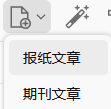
\includegraphics[width=0.4\linewidth]{img/zotero/zotero_savebyhand} 

}

\caption{手动添加}\label{fig:zotero-savebyhand}
\end{figure}

\subsection{对文献条目的引用}\label{ux5bf9ux6587ux732eux6761ux76eeux7684ux5f15ux7528}

\subsubsection{生成指定文献的参考文献格式:}\label{ux751fux6210ux6307ux5b9aux6587ux732eux7684ux53c2ux8003ux6587ux732eux683cux5f0f}

右键点击所要生成参考文献的条目,选择``用所选条目创建参考文献表''。

\begin{figure}

{\centering 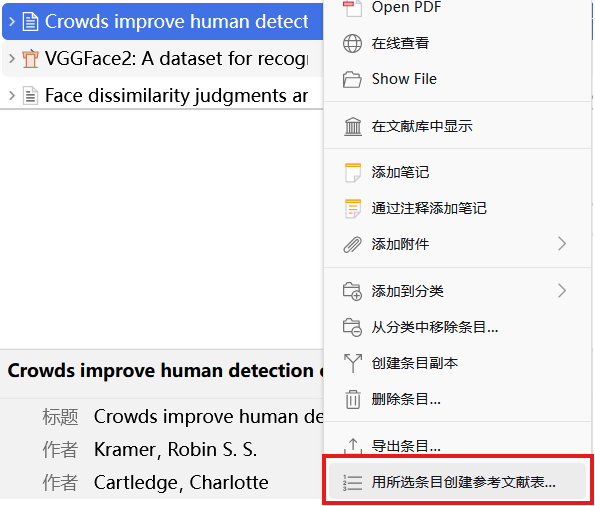
\includegraphics[width=0.7\linewidth]{img/zotero/zotero_reference_taxt_1} 

}

\caption{生成参考文献格式}\label{fig:zotero-reference-taxt-1}
\end{figure}

我们一般用APA7格式,点击 OK 复制到剪切板进行粘贴就好。

\begin{figure}

{\centering 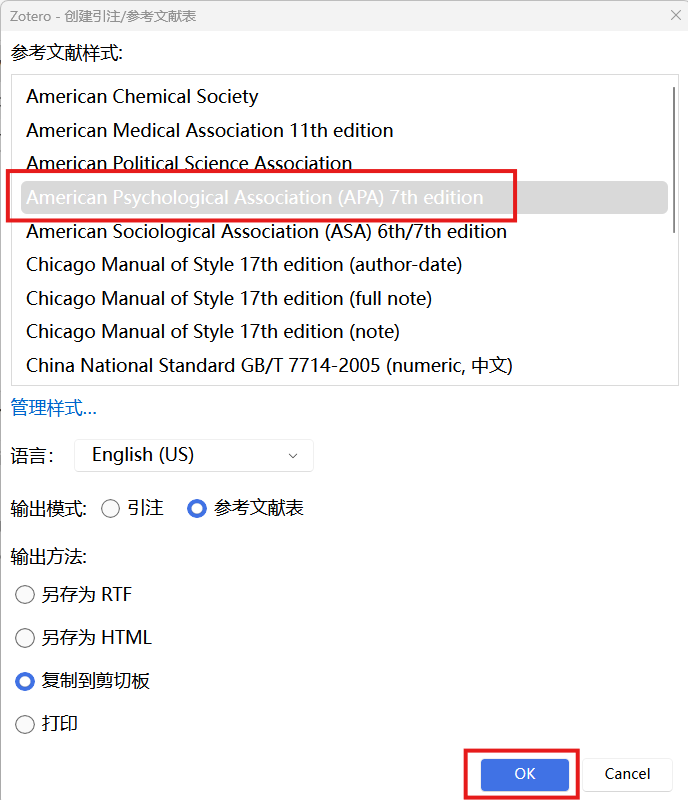
\includegraphics[width=0.7\linewidth]{img/zotero/zotero_reference_taxt_2} 

}

\caption{生成参考文献格式2}\label{fig:zotero-reference-taxt-2}
\end{figure}

\subsubsection{在文章中添加引用:}\label{ux5728ux6587ux7ae0ux4e2dux6dfbux52a0ux5f15ux7528}

Zotero的Word插件允许用户直接从Word中插入引文信息。通过进入Word上方工具栏中的``Zotero'',点击Add/Edit Citation来使用,而后在出现的输入框中搜索确定要插入的文献。这个功能使我们在写文章时可以很方便的随时引用多个文献信息。对于文本、脚注和尾注的引用都是支持的。

\subsubsection{自动生成参考文献书目:}\label{ux81eaux52a8ux751fux6210ux53c2ux8003ux6587ux732eux4e66ux76ee}

使用Zotero在Word中的插件点击Add/Edit Bibliography可以根据引用的文献自动生成参考书目。

\begin{figure}

{\centering 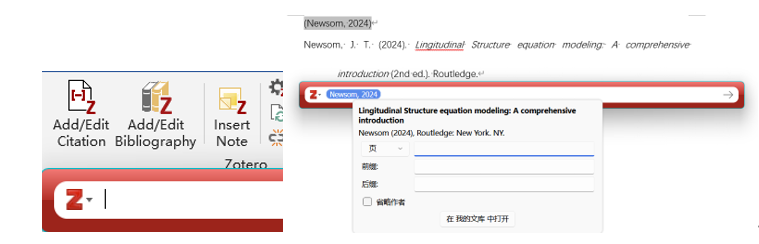
\includegraphics[width=1\linewidth]{img/zotero/zotero_citation} 

}

\caption{添加引文}\label{fig:zotero-citation}
\end{figure}

\subsection{同步与小组协作功能}\label{ux540cux6b65ux4e0eux5c0fux7ec4ux534fux4f5cux529fux80fd}

\subsubsection{数据同步:}\label{ux6570ux636eux540cux6b65}

Zotero可以在多台计算机中同步用户数据。库中的条目和笔记通过Zotero服务器同步。同步到Zotero服务器的条目可以通过zotero.org帐户在线访问。并且还可以与他人共享自己的数据库,或根据选定的条目创建自定义简历。在zotero.org上为读者、公众和其他使用自己出版物或发表的期刊的研究人员提供研究副本。

\subsubsection{小组文库:}\label{ux5c0fux7ec4ux6587ux5e93}

Zotero用户可以创建协作或兴趣小组。通过共享的小组数据库,我们可以通过在线的和通过Zotero客户端来协作管理研究资源和材料。

\begin{figure}

{\centering 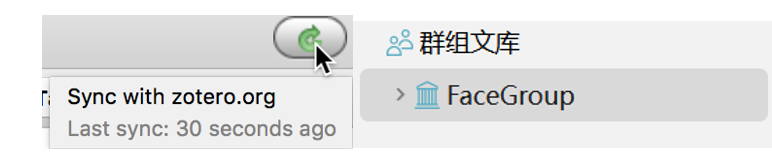
\includegraphics[width=1\linewidth]{img/zotero/zotero_groupwork} 

}

\caption{小组}\label{fig:zotero-groupwork}
\end{figure}

\section{拓展插件}\label{ux62d3ux5c55ux63d2ux4ef6}

\subsection{插件安装方法(也可直接参考文章开头推荐的博客)}\label{ux63d2ux4ef6ux5b89ux88c5ux65b9ux6cd5ux4e5fux53efux76f4ux63a5ux53c2ux8003ux6587ux7ae0ux5f00ux5934ux63a8ux8350ux7684ux535aux5ba2}

点击链接,进入\href{https://zotero-chinese.com/plugins/}{Zotero 插件商店}

选择与自己对于的版本,筛选类型或者直接搜索插件进行下载。

\begin{figure}

{\centering 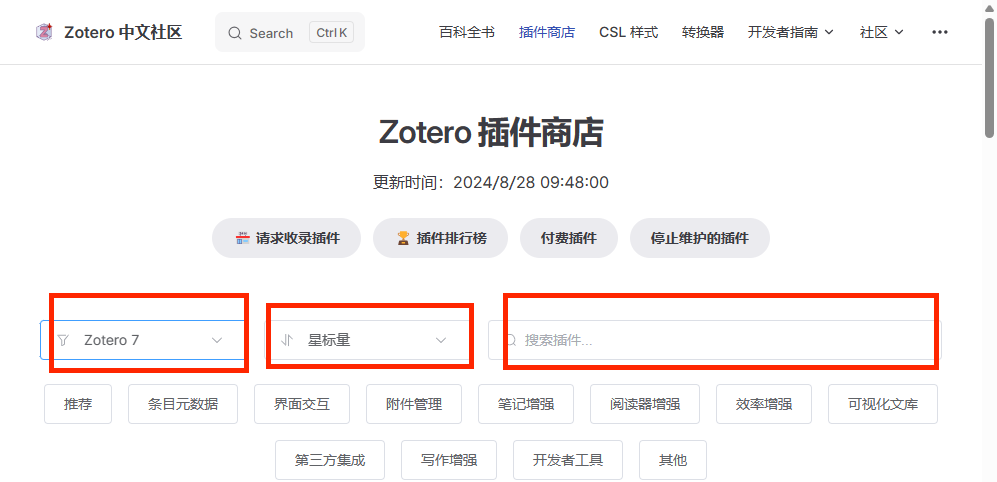
\includegraphics[width=0.7\linewidth]{img/zotero/zotero_plugins_interface} 

}

\caption{插件商店}\label{fig:zotero-plugins-interface}
\end{figure}

\begin{figure}

{\centering 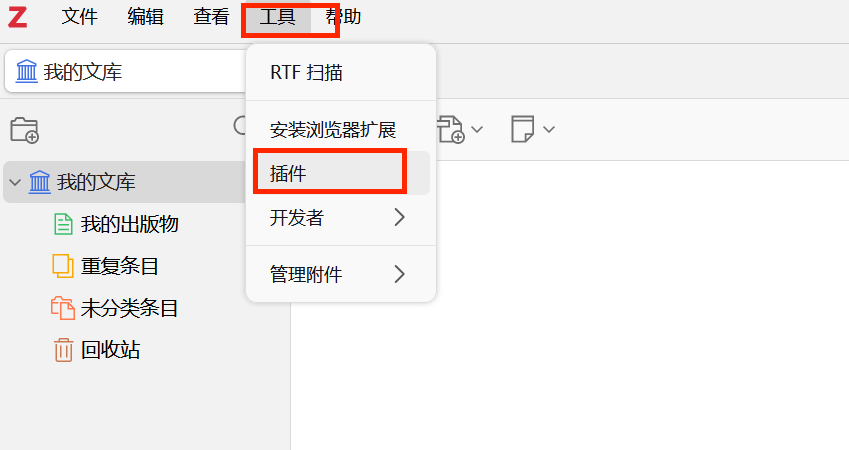
\includegraphics[width=0.7\linewidth]{img/zotero/zotero_plugins_install_1} 

}

\caption{插件安装1}\label{fig:zotero-plugins-install-1}
\end{figure}

将下载的插件(.xpi文件)拖拽进Manage Your Pligins界面即可安装成功。(注意版本对应)

\begin{figure}

{\centering 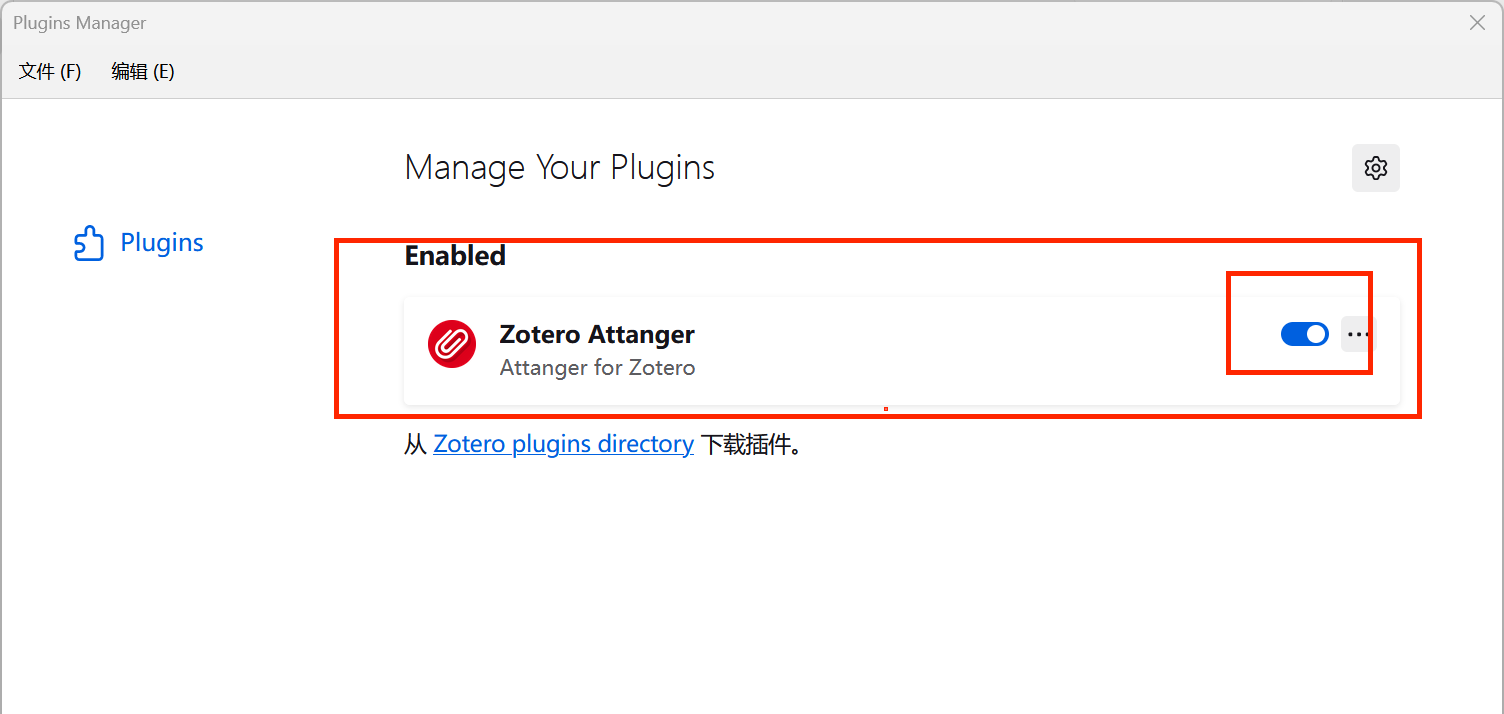
\includegraphics[width=0.7\linewidth]{img/zotero/zotero_plugins_install_2} 

}

\caption{插件安装2}\label{fig:zotero-plugins-install-2}
\end{figure}

\subsection{常用插件推荐}\label{ux5e38ux7528ux63d2ux4ef6ux63a8ux8350}

可根据自身需求进行安装。

\textbf{1.Jasminum 茉莉花(必装,后面在Word中文献引用时非常实用,但有时年份可能会有点错误,注意一下)}

支持中文题录信息下载,结合pdftk还可以为论文的PDF文件添加书签。能够抓取CNKI、万方、维普、百度学术等中文网址的资源,同时支持CAJ格式,等功能。

\textbf{2.Translate for Zotero}

将PDF、EPub、网页、元数据、注释、注解翻译为目标语言,支持20多种翻译服务。特别适合英文文献阅读 ,可实现将pdf中选中的文字翻译为指定语言,并将译文显示在弹窗或右侧的选项卡窗口中。

\textbf{3.Better BibTex for Zotero}

直接从知网、谷歌学术等抓取参考文献信息,并下载PDF保存在Zotero的文献库中。自动生成reference.bib文件,并与文献库内容保持同步更新。特别适用于LaTeX写论文,能让Zotero和LaTeX更好地搭配使用进行文献引用。(用LaTeX写论文也可以研究一下)

\textbf{4.Better Notes for Zotero}

集成了所有关于笔记管理的功能,支持主笔记创建、其他笔记链接、模板使用等,插件提供丰富的自定义选项,用户可以根据自己的需求调整界面布局和功能配置,插件支持Markdown格式,用户可以在Zotero内部与外部Markdown文件之间实现自动同步; 提供了多样化的笔记模板,让数据整理变得简单快捷,支持批量操作,减少重复劳动。

\textbf{5.Ethereal Style}

支持标签建立、网络图谱构建、进度可视化等功能。可以解决Zotero不显示标签文字的问题,显示阅读进度和标注进度,自定义作者列显示格式,修改PDF底色等。

\textbf{6.NoteroEthereal Reference}

自动识别文献的参考文献,并将其显示在右侧栏目,点击加号可直接添加到Zotero管理器中,无需打开网页。

\textbf{7.Green Frog}

从easyScholar更新期刊信息,获取期刊或会议论文的JCR分区、中科院分区、影响因子等信息。

\href{https://blog.csdn.net/tyutwuxuan/article/details/143827364?ops_request_misc=&request_id=&biz_id=102&utm_term=zotero\%E4\%B8\%8Eeasyscholar&utm_medium=distribute.pc_search_result.none-task-blog-2~all~sobaiduweb~default-0-143827364.142\%5Ev101\%5Econtrol&spm=1018.2226.3001.4187}{配置方法}可以参考链接中博客的教程。

\textbf{8.PDF Figure}

在PDF内实现图表解析和注释。

\textbf{9.zotxt}

文本扩展插件,用于文本编辑和扩展功能。

\textbf{10.Awesome GPT}

实现Zotero和ChatGPT的联动,更快更好地进行阅读和管理文献。

\part{其他工具}\label{part-ux5176ux4ed6ux5de5ux5177}

\chapter{Visual Studio Code}\label{vscode}

\section{下载安装}\label{ux4e0bux8f7dux5b89ux88c5-1}

请在\href{https://code.visualstudio.com/}{Visual Studio Code官网}下载该软件。

\section{制作公开数据的README.md文件}\label{mkreadme}

更新于:2024-11-29

\begin{enumerate}
\def\labelenumi{\arabic{enumi}.}
\tightlist
\item
  在Visual Studio Code中新建一个文本文档:
\end{enumerate}

\begin{figure}

{\centering 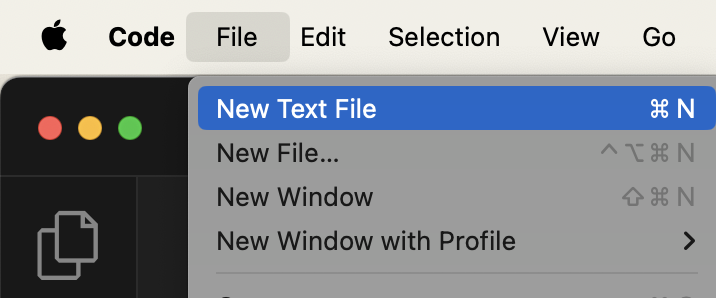
\includegraphics[width=0.6\linewidth]{img/vscode/mkreadme_mknewfile} 

}

\caption{在VS Code中新建一个文本文档}\label{fig:mkreadme-mknewfile}
\end{figure}

之后,你应该看到类似的新建文件:

\begin{figure}

{\centering 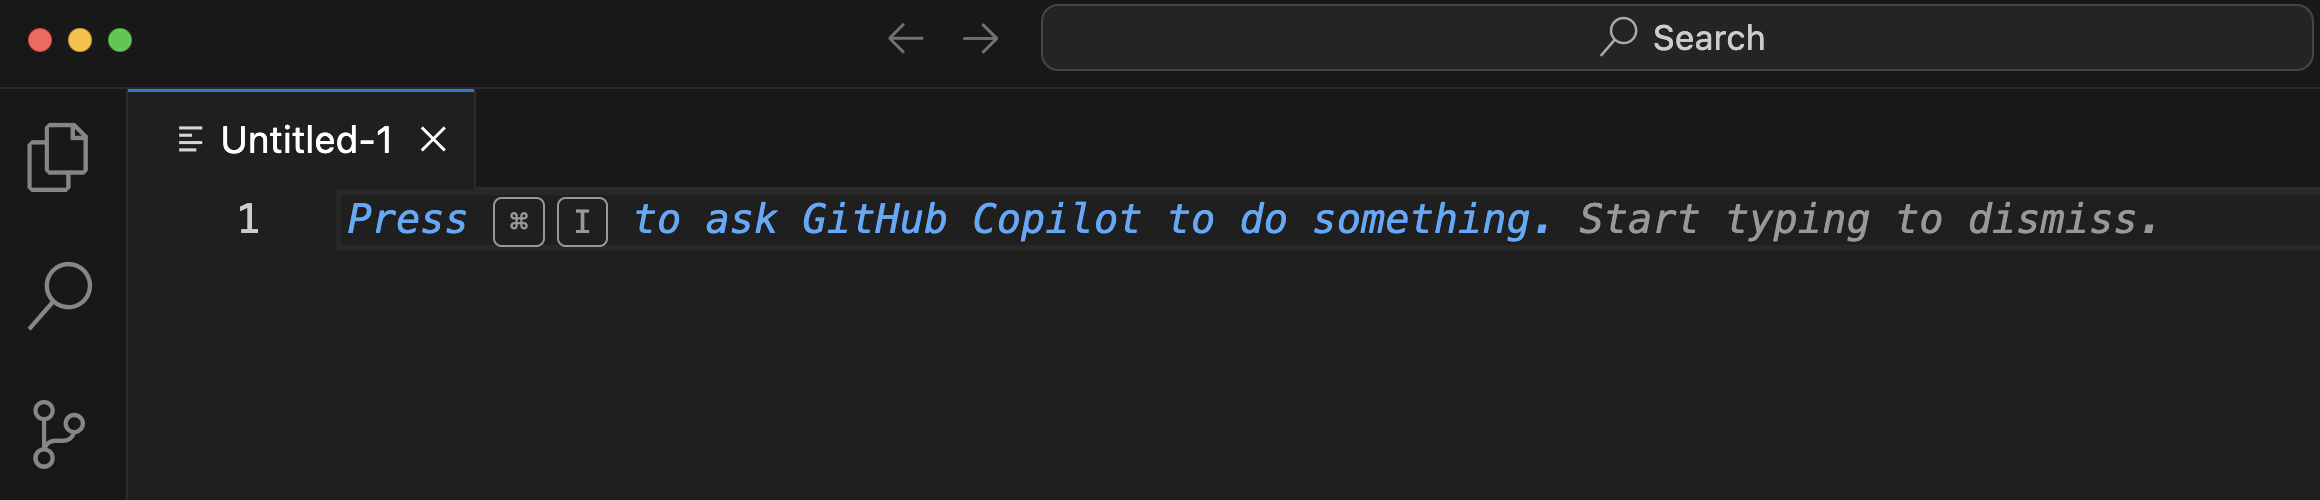
\includegraphics[width=1\linewidth]{img/vscode/mkreadme_newfile} 

}

\caption{VS Code中的新建文本文档}\label{fig:mkreadme-newfile}
\end{figure}

2. 将新建文档保存为\texttt{README.md}文件:

\begin{figure}

{\centering 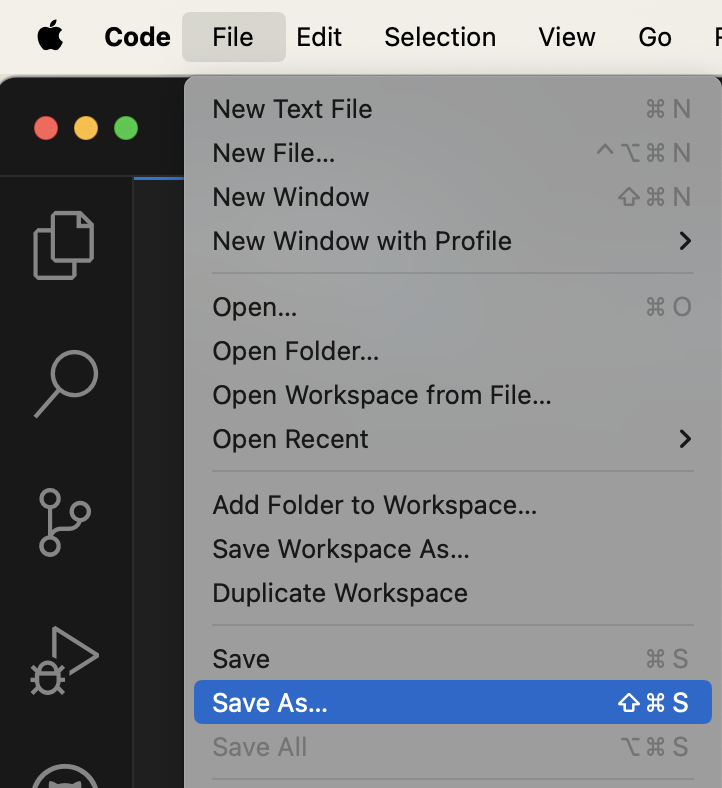
\includegraphics[width=0.7\linewidth]{img/vscode/mkreadme_saveas1} 

}

\caption{将新建文本文档另存为...}\label{fig:mkreadme-saveas1}
\end{figure}

在打开的对话框中,请选择保存新建文本文档的位置,并将文件命名为\texttt{README.md}:

\begin{figure}

{\centering 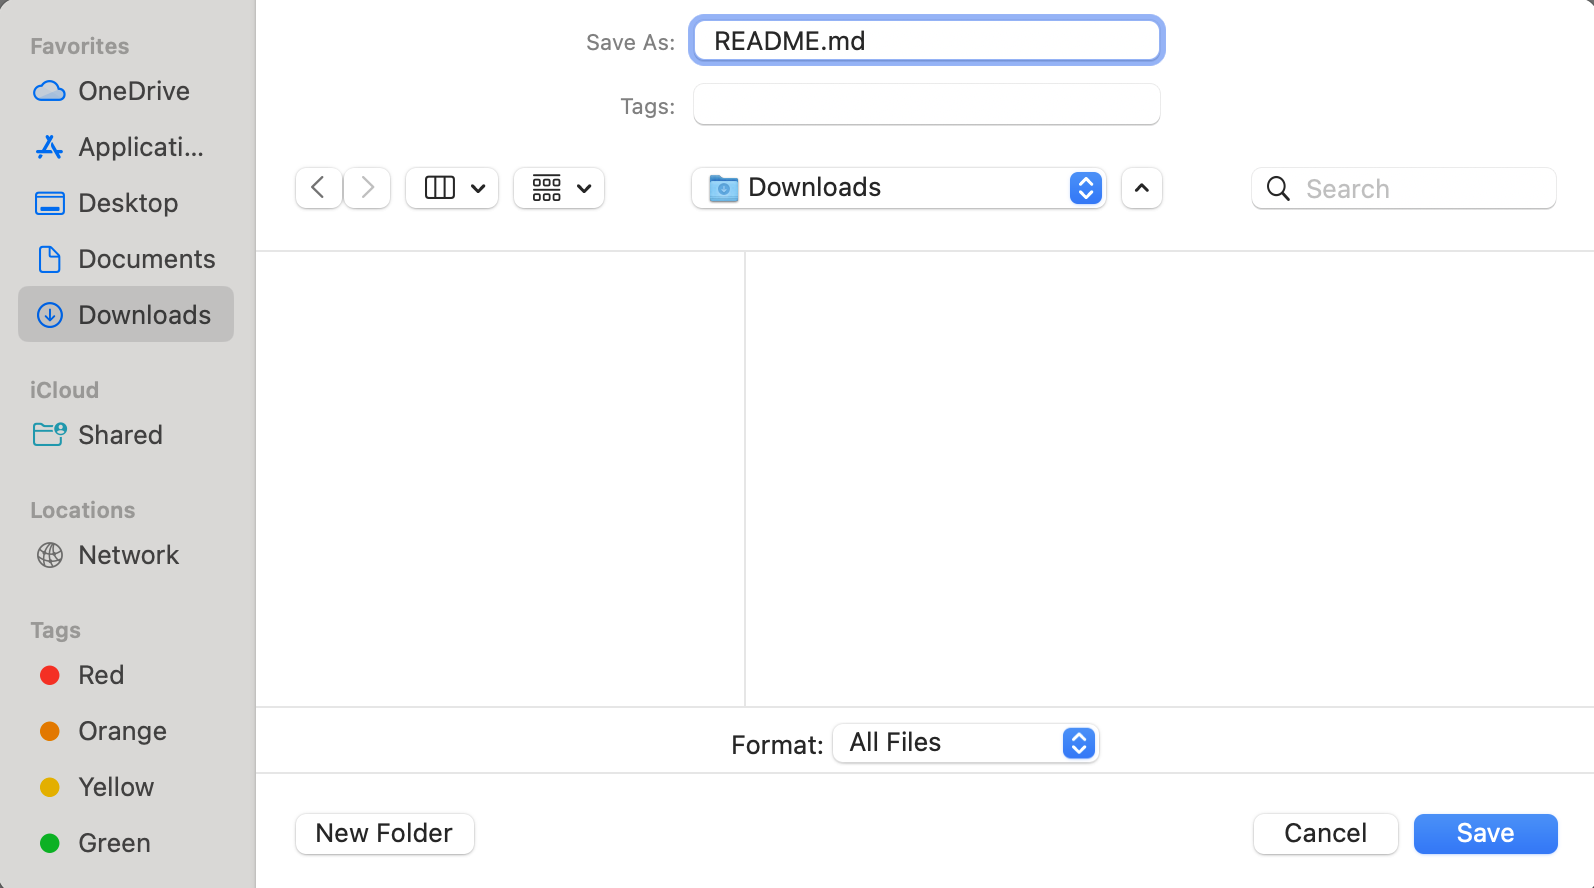
\includegraphics[width=0.8\linewidth]{img/vscode/mkreadme_saveas2} 

}

\caption{重命名文件为“README.md”并选择文件存储位置}\label{fig:mkreadme-saveas2}
\end{figure}

3. 根据数据文件编辑\texttt{README.md}文件

在\texttt{README.md}文件中,你可以添加根据数据文件的内容,添加列名称(\texttt{Header})和内容描述(\texttt{Description}):

\begin{Shaded}
\begin{Highlighting}[]

\NormalTok{Header | Description}
\NormalTok{{-}{-}{-}|{-}{-}{-}}
\NormalTok{Column1 | Description of Column1}
\NormalTok{Column2 | Description of Column2}
\end{Highlighting}
\end{Shaded}

假定我们用有这样一个数据文件:

\begin{figure}

{\centering 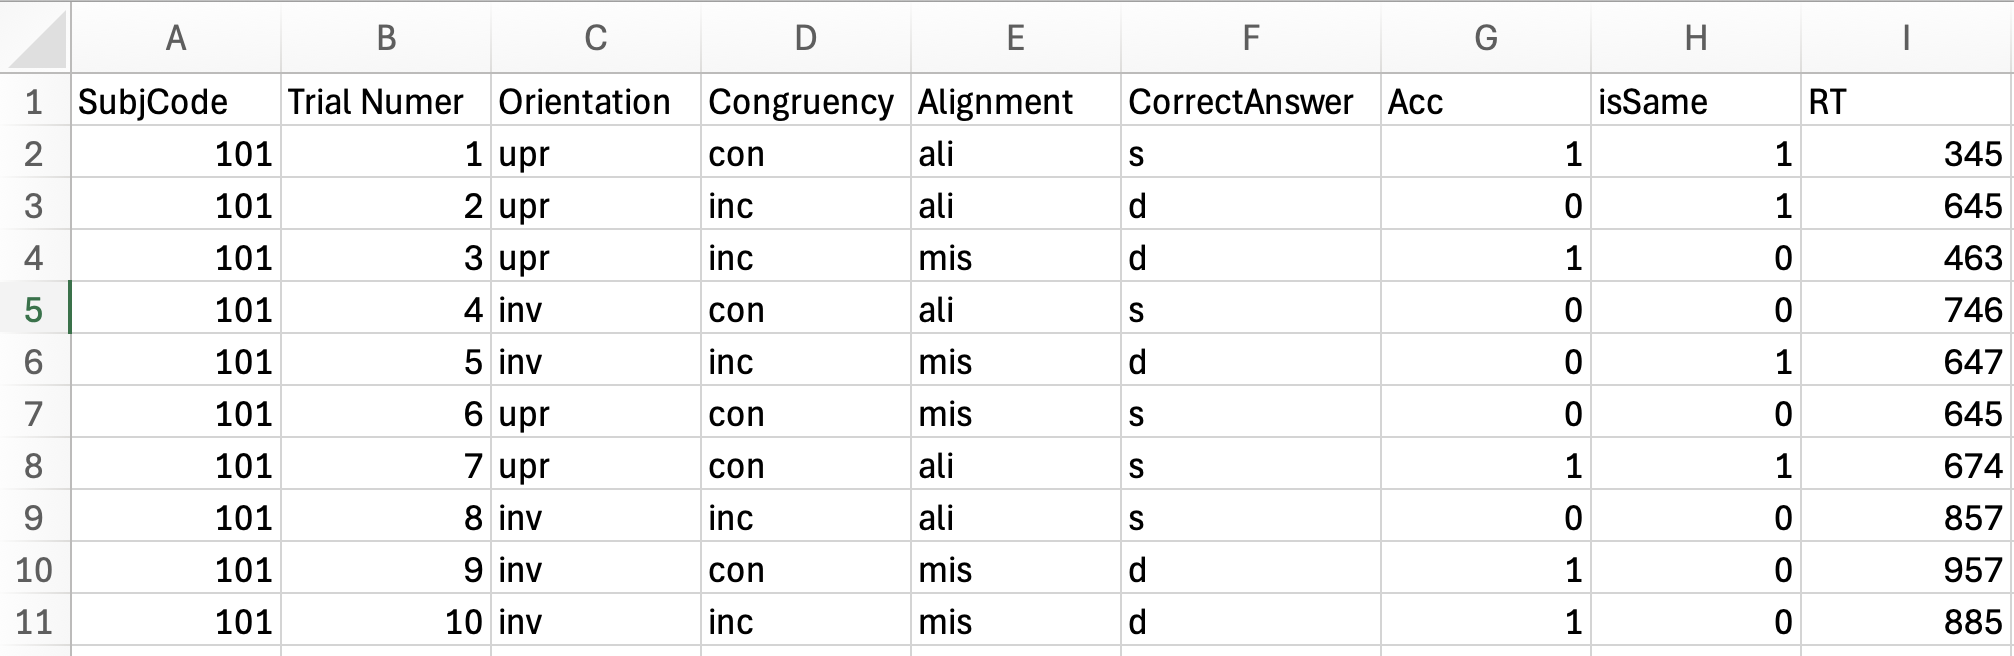
\includegraphics[width=1\linewidth]{img/vscode/mkreadme_datafile} 

}

\caption{数据文件}\label{fig:mkreadme-datafile}
\end{figure}

我们相应地编辑\texttt{README.md}文件:

\begin{Shaded}
\begin{Highlighting}[]

\NormalTok{Header | Description}
\NormalTok{{-}{-}{-}|{-}{-}{-}}
\NormalTok{SubjCode | Subject Code}
\NormalTok{Trial Number | trial number}
\NormalTok{Orientation | orientation of the stimulus: }\InformationTok{\textasciigrave{}upr\textasciigrave{}}\NormalTok{: upright vs }\InformationTok{\textasciigrave{}inv\textasciigrave{}}\NormalTok{: inverted}
\NormalTok{Congruency | congruency of the trial type in complete composite task: }\InformationTok{\textasciigrave{}con\textasciigrave{}}\NormalTok{: congruent vs }\InformationTok{\textasciigrave{}inc\textasciigrave{}}\NormalTok{: incongruent}
\NormalTok{Alignment | whether the top and bottom halves of faces are aligned (}\InformationTok{\textasciigrave{}ali\textasciigrave{}}\NormalTok{) or misaligned (}\InformationTok{\textasciigrave{}mis\textasciigrave{}}\NormalTok{)}
\NormalTok{CorrectAnswer | whether the correct response was the same (}\InformationTok{\textasciigrave{}s\textasciigrave{}}\NormalTok{) or different (}\InformationTok{\textasciigrave{}d\textasciigrave{}}\NormalTok{)}
\NormalTok{Acc | whether the response was correct (}\InformationTok{\textasciigrave{}1\textasciigrave{}}\NormalTok{) or incorrect (}\InformationTok{\textasciigrave{}0\textasciigrave{}}\NormalTok{)}
\NormalTok{isSame | whether participant reported the same (}\InformationTok{\textasciigrave{}1\textasciigrave{}}\NormalTok{) or not (}\InformationTok{\textasciigrave{}0\textasciigrave{}}\NormalTok{) for that trial}
\NormalTok{RT | response time in milliseconds}
\end{Highlighting}
\end{Shaded}

4. 编辑\texttt{README.md}文件的同时预览效果

在编辑\texttt{README.md}文件的同时,你可以通过以下方式来预览效果:

\begin{itemize}
\tightlist
\item
  \texttt{Ctrl\ +\ Shift\ +\ V} (Windows)快捷键
\item
  \texttt{Cmd\ +\ Shift\ +\ V} (Mac)快捷键
\item
  右键点击\texttt{README.md}文件,选择\texttt{Open\ Preview}选项
\end{itemize}

\begin{figure}

{\centering 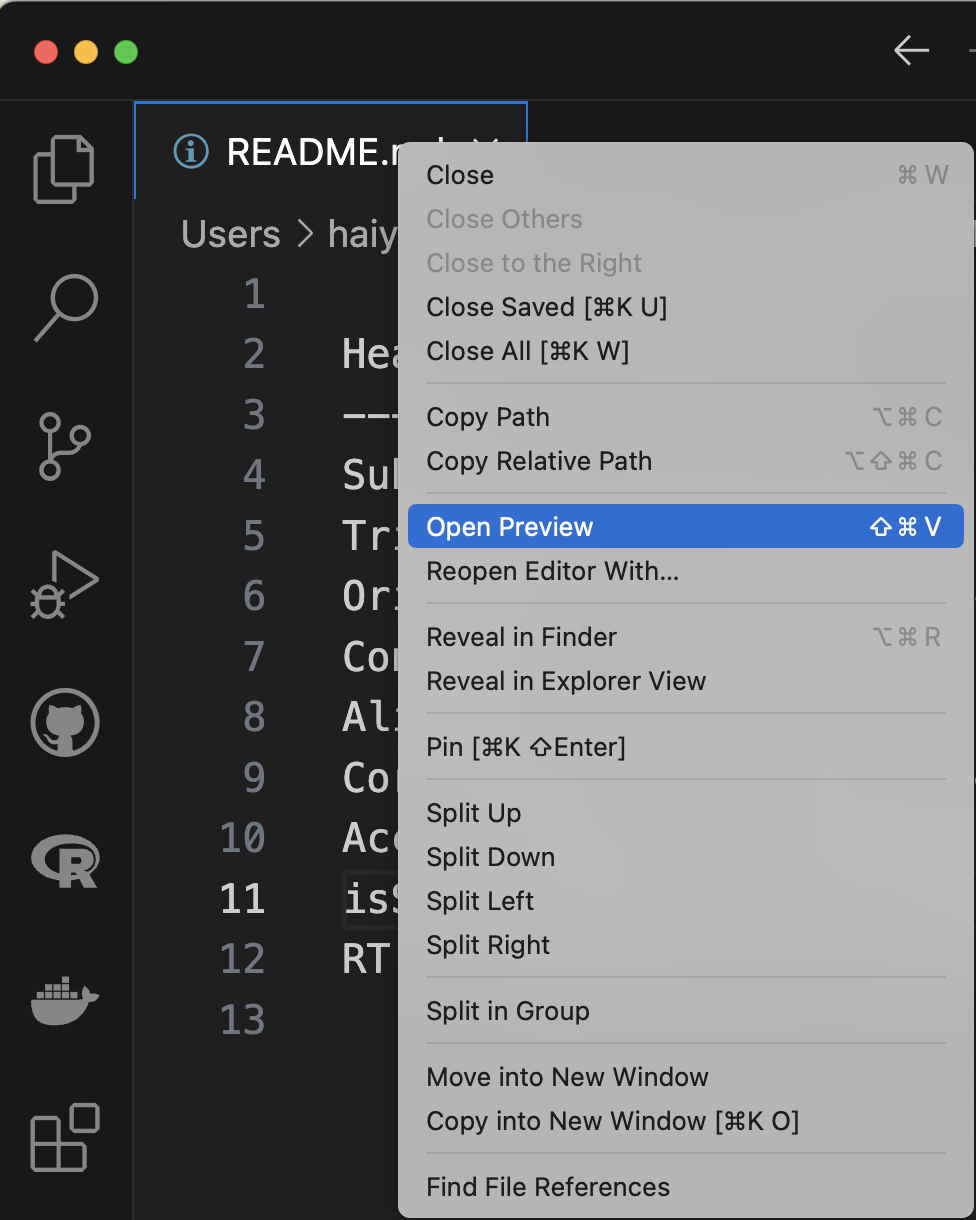
\includegraphics[width=0.6\linewidth]{img/vscode/mkreadme_openpreview} 

}

\caption{右键点击`README.md`文件,选择`Open Preview`选项}\label{fig:mkreadme-openpreview}
\end{figure}

预览效果与下图类似:

\begin{figure}

{\centering 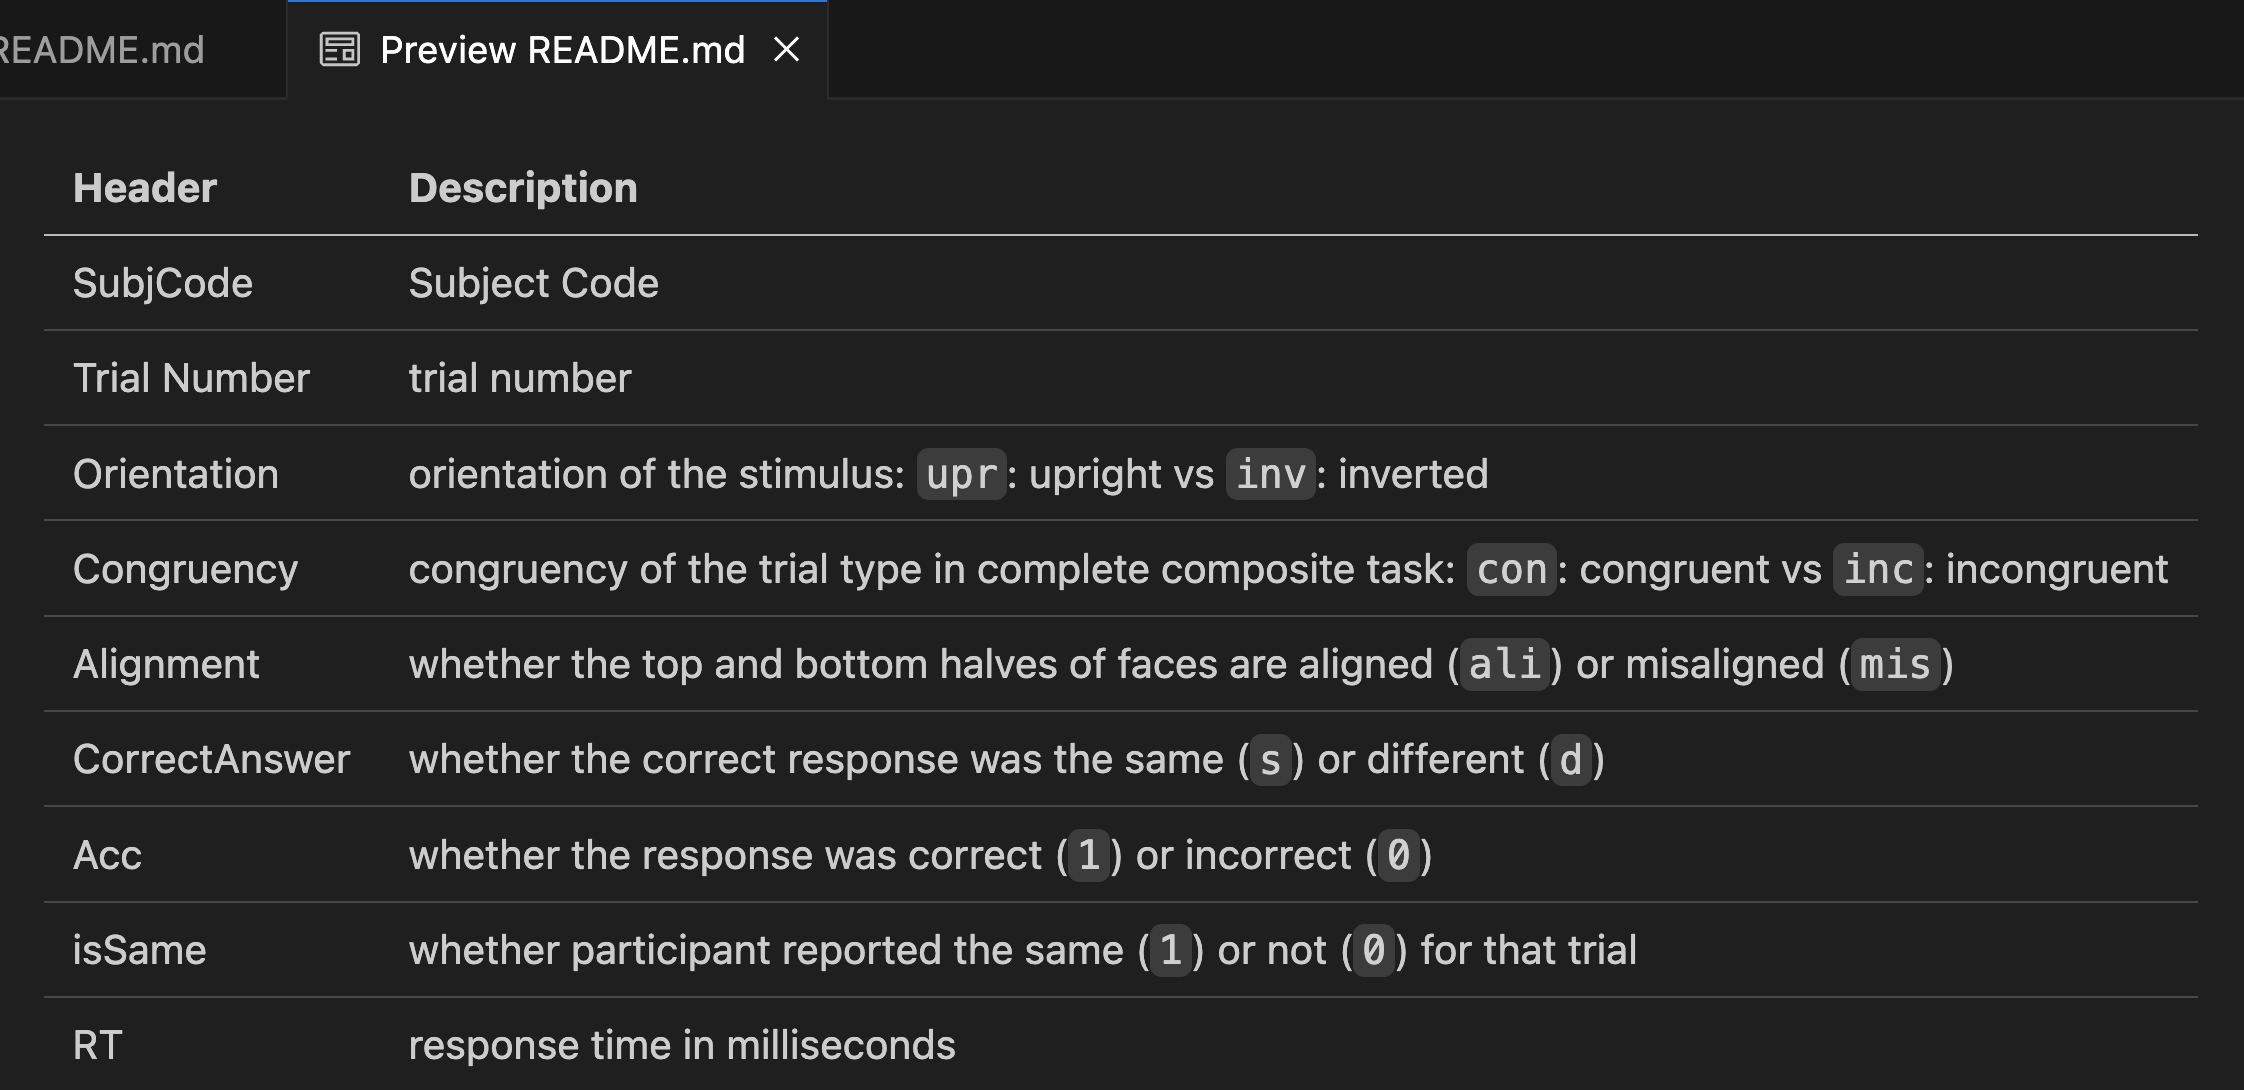
\includegraphics[width=1\linewidth]{img/vscode/mkreadme_preview} 

}

\caption{预览md文件}\label{fig:mkreadme-preview}
\end{figure}

5. 将\texttt{README.md}文件保存为pdf文件

完成编辑\texttt{README.md}文件后,我们可以将其保存为或生成一个pdf文档。

5.1 在VS Code中安装\texttt{Markdown\ PDF}插件

\begin{figure}

{\centering 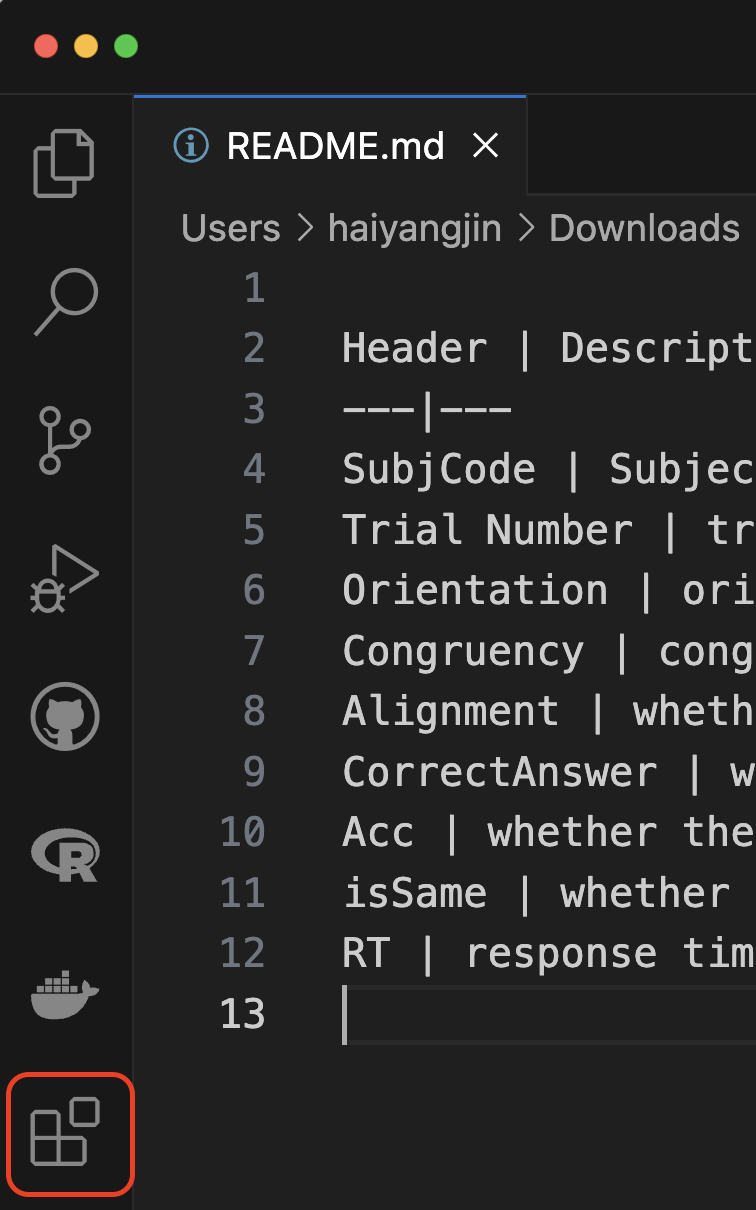
\includegraphics[width=0.4\linewidth]{img/vscode/mkreadme_extension} 

}

\caption{VS Code中打开Extension}\label{fig:mkreadme-extension}
\end{figure}

在搜索框中输入\texttt{Markdown\ PDF},并点击安装(\texttt{Install}):

\begin{figure}

{\centering 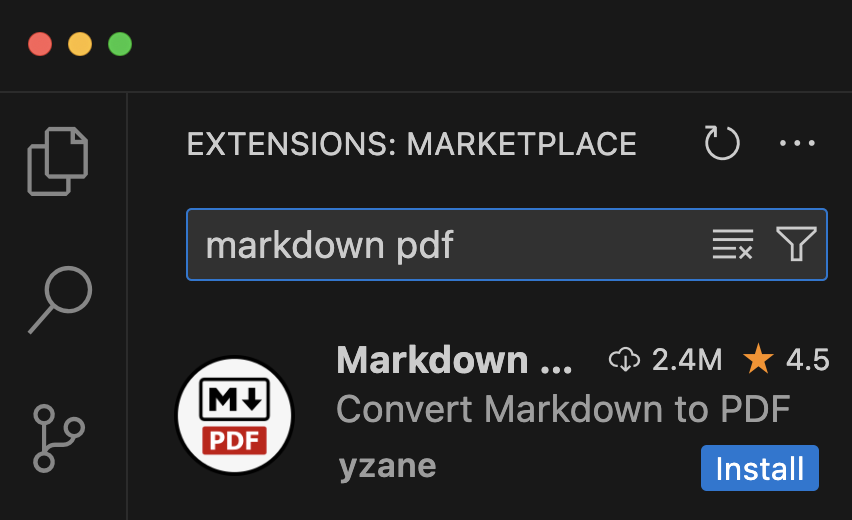
\includegraphics[width=0.5\linewidth]{img/vscode/mkreadme_markdownpdf} 

}

\caption{搜索并安装Markdown PDF}\label{fig:mkreadme-markdownpdf}
\end{figure}

5.2 生成pdf文件

安装完成\texttt{Markdown\ PDF}插件后,请确保\texttt{README.md}已在VS Code中打开,然后通过\texttt{View\ -\textgreater{}\ Command\ Palette}打开\texttt{Command\ Palette}:

\begin{figure}

{\centering 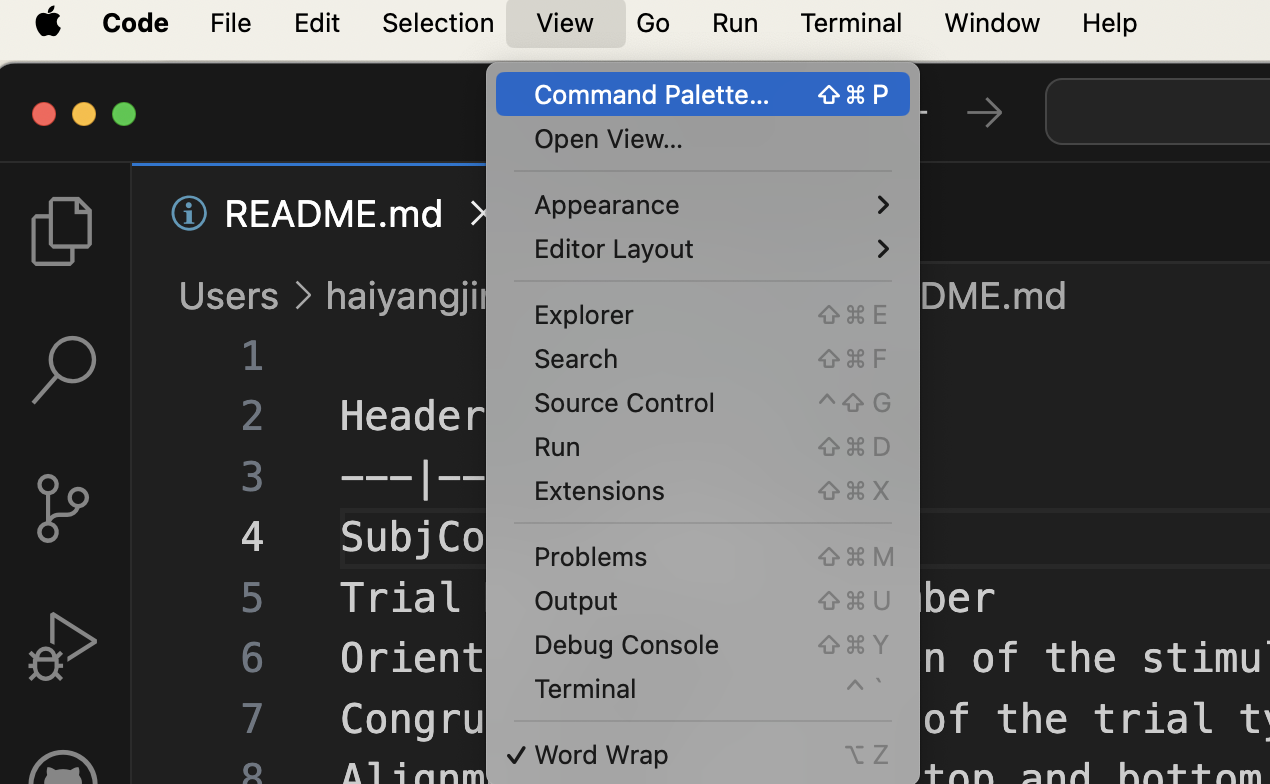
\includegraphics[width=0.75\linewidth]{img/vscode/mkreadme_palette} 

}

\caption{打开Command Palette}\label{fig:mkreadme-palette}
\end{figure}

然后在\texttt{Command\ Palette}中搜索并打开\texttt{Markdown\ PDF:\ Export\ (pdf)}:

\begin{figure}

{\centering 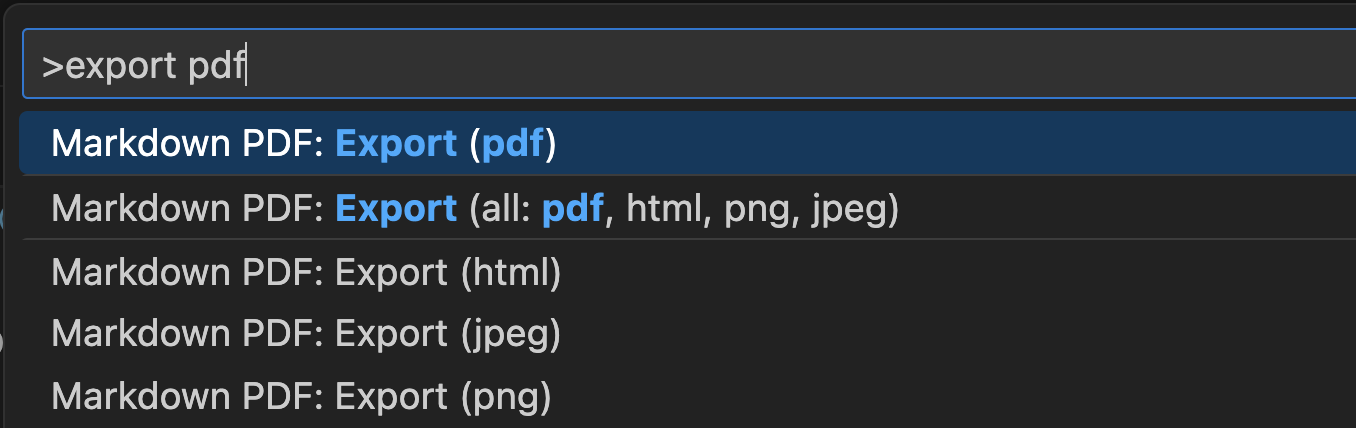
\includegraphics[width=0.6\linewidth]{img/vscode/mkreadme_exportpdf} 

}

\caption{Markdown PDF Export (pdf)}\label{fig:mkreadme-exportpdf}
\end{figure}

之后,你应该在VS Code右下角看到正在生成pdf文件的提示消息:

\begin{figure}

{\centering 
\includegraphics[width=0.8\linewidth]{img/vscode/mkreadme_exportmessage} 

}

\caption{正在生成PDF文件...}\label{fig:mkreadme-exportmessage}
\end{figure}

提示消息消失后,你可以在\texttt{README.md}文件所在的文件夹中找到生成的pdf文件:

\begin{figure}

{\centering 
\includegraphics[width=0.6\linewidth]{img/vscode/mkreadme_mkpdf} 

}

\caption{正在生成PDF文件...}\label{fig:mkreadme-mkpdf}
\end{figure}

生成的pdf文件效果如下:

\begin{figure}

{\centering \includegraphics[width=1\linewidth]{img/vscode/mkreadme_pdf} 

}

\caption{PDF文件}\label{fig:mkreadme-pdf}
\end{figure}

\chapter{One Drive}\label{onedrive}

汇总:郭沫然\\
更新于:2025-01-20

OneDrive是微软公司推出的文件和照片的云存储空间APP,常被用于同步盘。对于win10和win11系统,OneDrive已预装至计算机中。

OneDrive个人用户只有5G的免费云空间,高校学生和老师可通过学校邮箱申请微软账号获得100G的免费云空间。

\section{学生个人邮箱}\label{ux5b66ux751fux4e2aux4ebaux90aeux7bb1}

邮箱名为: \href{mailto:学号@mails.zstu.edu.cn}{\nolinkurl{学号@mails.zstu.edu.cn}}

登录密码和统一身份认证密码一致,先激活统一身份系统(SSO)账号后方可使用学生邮箱。

可以在\href{https://mailh.qiye.163.com}{网易企业邮箱}登陆来收发邮件。

\begin{figure}

{\centering \includegraphics[width=1\linewidth]{img/OneDrive/MailBox} 

}

\caption{MailBox}\label{fig:OneDrive-MailBox}
\end{figure}

\section{注册}\label{ux6ce8ux518c}

进入\href{https://www.microsoft.com/zh-cn/microsoft-365}{Microsoft 365}网站。

下滑至界面最底部,找到 ``Office 教育版'' 。

\begin{figure}

{\centering \includegraphics[width=1\linewidth]{img/OneDrive/Office_Education} 

}

\caption{OfficeEducation}\label{fig:OneDrive-OfficeEducation}
\end{figure}

进入后点击 ``开始使用'' 进入注册界面。

\begin{figure}

{\centering \includegraphics[width=1\linewidth]{img/OneDrive/Office_Education2} 

}

\caption{OfficeEducation2}\label{fig:OneDrive-OfficeEducation2}
\end{figure}

点击 ``我是学生'',开始创建账户。

\begin{figure}

{\centering \includegraphics[width=0.8\linewidth]{img/OneDrive/Register_1} 

}

\caption{Register1}\label{fig:OneDrive-Register1}
\end{figure}

填写学校个人邮箱,然后根据引导填写注册所需的信息以及邮箱验证码。在上面(``学生个人邮箱``那一节)提到的邮箱网址查看验证码。

\begin{figure}

{\centering \includegraphics[width=0.8\linewidth]{img/OneDrive/Register_2} 

}

\caption{Register2}\label{fig:OneDrive-Register2}
\end{figure}

\begin{figure}

{\centering \includegraphics[width=0.8\linewidth]{img/OneDrive/Register_3} 

}

\caption{Register3}\label{fig:OneDrive-Register3}
\end{figure}

邀请同事这一步不用管,点击 ``跳过并转到Office 365教育版'' 。

\begin{figure}

{\centering \includegraphics[width=0.8\linewidth]{img/OneDrive/Invitation} 

}

\caption{Invitation}\label{fig:OneDrive-Invitation}
\end{figure}

最后点击 ``开始'' 完成注册。

\begin{figure}

{\centering \includegraphics[width=0.8\linewidth]{img/OneDrive/RegisterEnd} 

}

\caption{RegisterEnd}\label{fig:OneDrive-RegisterEnd}
\end{figure}

\section{使用}\label{ux4f7fux7528}

通常Win10和Win11系统会自带OneDrive,在电脑里找到OneDrive(通常在任务栏右侧的 ``云朵'' 图标就是,如下图)打开登录。

\begin{figure}

{\centering \includegraphics[width=0.9\linewidth]{img/OneDrive/OneDrive_Icon} 

}

\caption{OneDrive Icon}\label{fig:OneDrive-OneDriveIcon}
\end{figure}

如果电脑上没有,或者电脑不是最新版OneDrive,也可以去\href{https://www.microsoft.com/en-us/microsoft-365/onedrive/download?ocid=ORSEARCH_Bing}{OneDrive官网}下载OneDrive最新版安装软件。

点击我的电脑,然后点击OneDrive,就会弹出登录界面,然后输入上面注册的账号就可以登录了。会弹出一个选择``个人''还是``工作或学校'',点击工作或学校,然后输入密码。

\textbf{注意:}记得选择自己想要保存到本地磁盘的位置,建议不要保存到C盘,例如E盘。

\begin{figure}

{\centering \includegraphics[width=1\linewidth]{img/OneDrive/Log_in} 

}

\caption{Log in}\label{fig:OneDrive-LogIn}
\end{figure}

随后会让你选择需要同步备份的文件夹,按自己的需要进行选择。

后期在设置的 ``同步并备份'' 中的 `` 管理备份'' 可以重新设置。

\begin{figure}

{\centering \includegraphics[width=1\linewidth]{img/OneDrive/Setting} 

}

\caption{Setting}\label{fig:OneDrive-Setting}
\end{figure}

在设置的 ``账户'' 中的 ``选择文件夹'' 中也可以选择在自己账户的OneDrive中可用的文件夹。

\begin{figure}

{\centering \includegraphics[width=1\linewidth]{img/OneDrive/ChooseFolders1} 

}

\caption{ChooseFolders1}\label{fig:OneDrive-ChooseFolders1}
\end{figure}

\begin{figure}

{\centering \includegraphics[width=1\linewidth]{img/OneDrive/ChooseFolders2} 

}

\caption{ChooseFolders2}\label{fig:OneDrive-ChooseFolders2}
\end{figure}

随后正常使用即可。

\subsection{更改OneDrive的保存位置}\label{ux66f4ux6539onedriveux7684ux4fddux5b58ux4f4dux7f6e}

\textbf{注意:}在进行更改保存位置操作前,记得关闭要备份文件中所有正在打开的内容,不然可能出现在更改位置后,有些文档被自动创建副本的现象。

\begin{figure}

{\centering \includegraphics[width=0.6\linewidth]{img/OneDrive/Error1} 

}

\caption{Error}\label{fig:OneDrive-Error1}
\end{figure}

打开OneDrive的设置,点击 ``取消链接此电脑'',确定 ``取消链接账户''。

\begin{figure}

{\centering \includegraphics[width=1\linewidth]{img/OneDrive/ChangeAddress1} 

}

\caption{ChangeAddress1}\label{fig:OneDrive-ChangeAddress1}
\end{figure}

然后重新登陆你的OneDrive帐号,在显示选择保存位置的页面点击 ``更改位置'' 选择要保存到的地址。

\begin{figure}

{\centering \includegraphics[width=1\linewidth]{img/OneDrive/ChangeAddress2} 

}

\caption{ChangeAddress2}\label{fig:OneDrive-ChangeAddress2}
\end{figure}

然后等待文件重新备份就可以了。(需要一点耐心)

\subsection{网页登陆}\label{ux7f51ux9875ux767bux9646}

可以在自己的OneDrive中找到 ``在线查看'',随后就会自动打开浏览器在线查看已备份的文档。

\begin{figure}

{\centering \includegraphics[width=0.9\linewidth]{img/OneDrive/Online1} 

}

\caption{Online1}\label{fig:OneDrive-Online1}
\end{figure}

也可以进入\href{https://www.microsoft.com/en-us/microsoft-365/onedrive/online-cloud-storage}{OneDrive官网}登陆在线查看(或许需要科学上网)。

在线登录方便跨设备查看。

\part{实验材料和公开数据}\label{part-ux5b9eux9a8cux6750ux6599ux548cux516cux5f00ux6570ux636e}

\chapter{实验材料}\label{materials}

汇总:\\
更新于:

\section{Chicago Face Database (芝加哥面孔数据库)}\label{chicago-face-database-ux829dux52a0ux54e5ux9762ux5b54ux6570ux636eux5e93}

\href{https://www.chicagofaces.org/}{Chicago Face Database}

Ma, D. S., Correll, J., \& Wittenbrink, B. (2015). The Chicago face database: A free stimulus set of faces and norming data. \emph{Behavior Research Methods}, 47(4), 1122--1135. \url{https://doi.org/10.3758/s13428-014-0532-5}

Ma, D. S., Kantner, J., \& Wittenbrink, B. (2021). Chicago Face Database: Multiracial expansion. \emph{Behavior Research Methods}, 53(3), 1289--1300. \url{https://doi.org/10.3758/s13428-020-01482-5}

\chapter{面孔加工能力测试}\label{facetest}

汇总:郭沫然\\
更新于:2024-12-16

\section{格拉斯哥面孔匹配测试}\label{ux683cux62c9ux65afux54e5ux9762ux5b54ux5339ux914dux6d4bux8bd5}

格拉斯哥面孔匹配测试(Glasgow Face Matching Test, GFMT)

\begin{enumerate}
\def\labelenumi{\arabic{enumi}.}
\tightlist
\item
  GFMT (Long) 包括168对面孔每个张面孔为全脸图像、中性表情。
\item
  所有的图像均在同一背景拍摄,距离为90厘米。\\
\item
  两张图像的拍摄间隔大约为15分钟每个身份面孔,分别使用相机(相机1:富士FinePix0800Zoom, 600万像素)拍摄的全脸图像;摄像机(相机2:松下NV-DS29B DS29)拍摄的相同姿势并取其中一帧图像。\\
\item
  所有的图像沿头部周围整齐裁剪,删除背景和衣服,大小调整为350像素宽,以72 ppi的分辨率灰度存储。\\
\item
  测试构建成对的刺激时,两面孔图像中鼻梁间水平距离为500像素有一半是同脸试次,同一人的两张图像并排呈现,这84身份面孔也被用于不同面孔的试次,与数据库中一张相似面孔匹配呈现。\\
\item
  GFMT (Short) 只包含40对面孔这个测试的项目从完整版本中最难的项目选取选出了导致错误最多的20对匹配项目和20对不匹配项目
\end{enumerate}

\section{格拉斯哥面孔匹配测试2}\label{ux683cux62c9ux65afux54e5ux9762ux5b54ux5339ux914dux6d4bux8bd52}

格拉斯哥面孔匹配测试2(Glasgow Face Matching Test 2, GFMT2)

\begin{enumerate}
\def\labelenumi{\arabic{enumi}.}
\tightlist
\item
  GFMT2使用与GFMT相同的图像来源-格拉斯哥不熟悉面孔数据库(Glasgow Unfamiliar Face Database, GUFD)构建。\\
\item
  所有匹配和不匹配的配对都不同于GFMT中使用的配对。\\
\item
  对每一个原始面孔身份分别创建三种不同变化材料:使用单反相机捕获头部角度刚性变化的静态图像;使用摄像机记录被试在说话和做出手势时面部运动的非刚性变化;从视频记录中采样包含姿势和头部角度轻微变化的图像,被试距离相机2米(原90厘米),从而引入相机到被试的距离变化分别对每一个变化图像进行配对。\\
\item
  GFMT2简短版本(GFMT2-S)不包含重复的面部身份,只包含三种变化中的一种配对,包括两个难度相同的40项测试表格, GFMT2-sa和GFMT2-sb,共80项。\\
\item
  使用彩色图像。
\end{enumerate}

\section{肯特面孔匹配测试}\label{ux80afux7279ux9762ux5b54ux5339ux914dux6d4bux8bd5}

肯特面孔匹配测试(Kent Face Matching Test, KFMT)

\begin{enumerate}
\def\labelenumi{\arabic{enumi}.}
\tightlist
\item
  使用材料来自肯特大学面孔数据库(Kent University Face Database, KUFD)。\\
\item
  在实验室拍摄的面孔照片,中性表情(用摄像机记录下被试旋转头部向不同方向看的过程)。\\
\item
  相应被试的ID照片ID照片不受表情、姿势或图像捕捉设备的限制,为变异性的重要来源ID照片在实验室照片拍摄前至少三个月获得实验室照片和ID照片之间的平均时间间隔约为8.8个月。\\
\item
  KFMT(Short) 由来自KUFD的40对高加索身份面孔对(20对男20对女)组成每对面孔由一张实验室照片和一张ID照片组成这些实验室照片被裁剪成只包含头部和肩部,缩放为283x332像素的大小,分辨率为72ppi,并被放置在白色背景右侧ID照片的尺寸为142x192像素,分辨率为72ppi,放置在背景的左侧。\\
\item
  在KFMT的简短版本的40对图像中,20对为相同的身份;20对不同的身份,根据头发颜色、面部和眉毛形状方面的视觉相似性进行配对
\end{enumerate}

\section{伦敦面孔匹配测试}\label{ux4f26ux6566ux9762ux5b54ux5339ux914dux6d4bux8bd5}

模特面孔匹配测试(Models Face Matching Test, MFMT)

\begin{enumerate}
\def\labelenumi{\arabic{enumi}.}
\tightlist
\item
  135名男性模特的180张全彩图片,从一个专业模特作品集网站上获取。\\
\item
  图像均为正面面孔,被裁剪为只显示面部图像以300 × 420像素的大小以彩色呈现。\\
\item
  180张全彩图像被分为45个匹配试验和45个不匹配试验这些配对是通过6个人根据感知到的相似性将384张男性模特的面部图像分类成堆来预先确定的。\\
\item
  从所有试次中选出90个最困难的试验,并将它们分成三个独立但相同难度的部分,每个部分包含15个匹配和15个不匹配的试验。\\
\item
  对于MFMT (Long),每名被试完成所有三个部分每个部分使用的刺激是平衡的,即整个实验中,每个面孔对在三个区块中出现的频率相同
\end{enumerate}

\section{牛津面孔匹配测试}\label{ux725bux6d25ux9762ux5b54ux5339ux914dux6d4bux8bd5}

牛津面孔匹配测试(Oxford Face Matching Test, OFMT)

\begin{enumerate}
\def\labelenumi{\arabic{enumi}.}
\tightlist
\item
  从多个公开数据库中选取成对的面孔刺激所有的数据库都包含面孔对是同一个人还是不同人的信息。\\
\item
  面孔均为自然状态,年龄和性别各异,白种人,正面面孔,有头发,没有背景戴眼镜的照片被排除在外。\\
\item
  图片被裁剪成3:4的比例,确保刺激大部分面积为面孔这些图像通过人脸识别算法进行相似性评估匹配,并以灰度图像呈现给被试。\\
\item
  对于OFMT (Long),成对面孔刺激在1600毫秒内并排呈现,被试在1(非常不相似)到100(非常相似)的范围内判断这些面孔的相似性,以及明确判断面孔图像是否来自同一个人所有刺激使用标准呈现时间(不是根据被试的反应进行测试)。\\
\item
  用十对刺激作为注意力检测试次,用完全相同的面孔图像构建了五组相同的配对,同时用不同性别的面孔图像构建了五组不同的配对(针对人类被试)
\end{enumerate}

\section{专家化面孔匹配测试}\label{ux4e13ux5bb6ux5316ux9762ux5b54ux5339ux914dux6d4bux8bd5}

专家化面孔匹配测试(Expertise in Facial Comparison Test, EFCT)

\begin{enumerate}
\def\labelenumi{\arabic{enumi}.}
\tightlist
\item
  该测试材料来自不同环境条件下的自然面孔图像的面孔图像数据集该数据集专门用于在具有挑战性的条件下测试面孔识别算法,或针对具有面孔识别相关专业知识和经验的人群(例如:法医)。\\
\item
  面孔均为正面图像,所有面孔图像在对照明、表情和外观等因素控制最小的情况下拍摄。\\
  3.根据人脸识别算法将面孔图像对依据匹配得分分为三个子集:``好'',``中等'',``差'', EFCT只包含来自``中等''和``差''两个部分的图像对。\\
\item
  被试在拍摄时间不同的两种条件下完成直立和倒立图像对的EFCT(人类被试)。\\
\item
  回答问题选项: (Ⅰ) 确定他们是同一个人; (Ⅱ) 认为他们是同一个人; (Ⅲ) 不知道; (Ⅳ) 认为他们是不同的人; (Ⅴ) 肯定他们是不同的人。 6. 总的来说,EFCT由168对图像组成 (一半相同,一半不同),其中一半分配给直立测试,一半分配给倒立测试
\end{enumerate}

\chapter{公开数据库}\label{opendata}

汇总:\\
更新于:

\section{磁共振(fMRI)}\label{ux78c1ux5171ux632ffmri}

\section{脑电(EEG)}\label{ux8111ux7535eeg}

\section{行为}\label{ux884cux4e3a}

\cleardoublepage

\appendix \addcontentsline{toc}{chapter}{\appendixname}


\chapter{如何为本手册作出贡献}\label{contribute}

如果你发现这个手册对你有帮助,欢迎你也贡献一份力量。如果你觉得这个手册没有什么用处,同样欢迎你提出建议,和我们一起来完善它。

\section{直接Pull Request}\label{ux76f4ux63a5pull-request}

如果你已经可以非常熟练地使用 Git 和 GitHub,那么你可以直接在 GitHub 上提交issues或Pull Request。

\section{简易教程}\label{ux7b80ux6613ux6559ux7a0b}

如果你对 Git 和 GitHub 不太熟悉,也请不到担心,你仍然可以通过本教程,学习如何完成一个可以成为本手册一部分的Rmd文件。完成后你只需将新创建的Rmd文档发送给我们,审核通过后该文档内容就会出现在\href{https://haiyangjin.github.io/labbook/}{本实验室手册}。

\subsection{下载示例}\label{ux4e0bux8f7dux793aux4f8b}

首先请下载\href{https://github.com/HaiyangJin/labbook/archive/refs/heads/mini.zip}{示例}。解压后你会看到一个名为\texttt{labbook-mini}的文件夹。

\begin{figure}

{\centering \includegraphics[width=0.7\linewidth]{img/contribute/mini_dir} 

}

\caption{The minimal example directory}\label{fig:contri-mini-dir}
\end{figure}

\subsection{安装R和RStudio}\label{ux5b89ux88c5rux548crstudio}

如果你还没有安装R和RStudio,请先根据\href{https://haiyangjin.github.io/rpsych-cn/intro.html\#prepare}{这里的信息}安装相关软件以及进行相应的设置。

安装完成后,请不要忘了\href{https://haiyangjin.github.io/rpsych-cn/intro.html\#mirror}{设置R包的镜像源}。

完成后请安装bookdown包,可以在RStudio中运行以下代码来实现:

\begin{Shaded}
\begin{Highlighting}[]
\FunctionTok{install.packages}\NormalTok{(}\StringTok{"bookdown"}\NormalTok{)}
\end{Highlighting}
\end{Shaded}

如果遇到问题,可以尝试查看这里的\href{https://haiyangjin.github.io/rpsych-cn/qacn.html\#qacn}{帮助信息}。

\subsection{打开labbook.Rproj}\label{ux6253ux5f00labbook.rproj}

请\textbf{直接}双击\texttt{labbook-mini}文件夹中的\texttt{labbook.Rproj}文件,这样你就可以在RStudio中打开这个项目。

\begin{quote}
请\textbf{直接}双击\texttt{labbook-mini}文件夹中的\texttt{labbook.Rproj}文件,这样你就可以在RStudio中打开这个项目。
\end{quote}

\begin{theorem}
请\textbf{直接}双击\texttt{labbook-mini}文件夹中的\texttt{labbook.Rproj}文件,这样你就可以在RStudio中打开这个项目。
\end{theorem}

打开后你会看到如下的界面:

\begin{figure}

{\centering \includegraphics[width=0.9\linewidth]{img/contribute/mini_rproj} 

}

\caption{The minimal example R project}\label{fig:contri-mini-rproj}
\end{figure}

\textcolor{red}{\textbf{特别注意}}:请确保如上图 \ref{fig:contri-mini-rproj}右上角所示,当前的项目名称是\texttt{labbook-mini}。如果不是,请点击\texttt{File} -\textgreater{} \texttt{Open\ project...},然后选择\texttt{labbook-mini}文件夹中的\texttt{labbook.Rproj}文件,重新打开该项目。

\subsection{确认示例可以运行}\label{ux786eux8ba4ux793aux4f8bux53efux4ee5ux8fd0ux884c}

现在我们可以尝试运行这个示例了。请在RStudio右上角找到\texttt{Build},然后点击\texttt{Build\ Book}。如果一切顺利,会跳出一个窗口,同时你应该会在RStudio的右上角看到:

\begin{figure}

{\centering \includegraphics[width=0.7\linewidth]{img/contribute/mini_build} 

}

\caption{Build book for the minimal example}\label{fig:contri-mini-build}
\end{figure}

如果你不小心关掉了跳出的窗口,你应该会看到在\texttt{labbook-mini}文件夹中生成了一个\texttt{\_book}子文件夹,里面包含了一个\texttt{index.html}文件。请双击这个文件通过浏览器打开,你会看到一个网页版的示例。

\subsection{创建一个新的Rmd文件}\label{ux521bux5efaux4e00ux4e2aux65b0ux7684rmdux6587ux4ef6}

现在我们可以开始创建一个新的Rmd文件来介绍你想贡献的内容了。比如你可以打开\texttt{20-new.Rmd}文件,然后将其另存为\texttt{66-your\_topic.Rmd}。请确保你的文件名中包含了你的主题,这样我们可以更容易地了解不同\texttt{Rmd}文件的内容。

例如,你可以输入这些内容:

\begin{Shaded}
\begin{Highlighting}[]
\FunctionTok{\# 我的主题}

\InformationTok{    汇总:最棒的我     }
\InformationTok{    更新于:很开心的今天(或者2024年11月11日)}

\InformationTok{    就是想分享一下今天的快乐。。。}

\FunctionTok{\#\# 加一个二级标题}


\FunctionTok{\#\#\# 需要放一张照片}

\SpecialStringTok{{-} }\NormalTok{添加图片方式一:}
\InformationTok{\textasciigrave{}\textasciigrave{}\textasciigrave{}\{r test{-}my{-}topic, echo=FALSE, fig.cap=\textquotesingle{}我的图片\textquotesingle{}, out.width=\textquotesingle{}60\%\textquotesingle{}, fig.align=\textquotesingle{}center\textquotesingle{}\}}
\InformationTok{knitr::include\_graphics(file.path("img", "jamovi", "anova.png"))}
\InformationTok{\textasciigrave{}\textasciigrave{}\textasciigrave{}}

\SpecialStringTok{{-} }\NormalTok{添加图片方式二:}
\AlertTok{![](img/jamovi/modules{-}library.png)}

\FunctionTok{\#\# 再给文字加一些颜料}

\NormalTok{随随便便放一些文字,看看效果如何。}

\NormalTok{我还想再给某一些文字加个链接,比如}\CommentTok{[}\OtherTok{这里}\CommentTok{](https://www.jamovi.org/)}\NormalTok{。}
\NormalTok{或者再加一些特定的颜色,比如}\CommentTok{[}\OtherTok{红色}\CommentTok{]}\NormalTok{\{color="red"\}和}\CommentTok{[}\OtherTok{蓝色}\CommentTok{]}\NormalTok{\{color="green"\},}
\CommentTok{[}\OtherTok{对的,}\CommentTok{]}\NormalTok{\{color="\#5bc0eb"\}}\CommentTok{[}\OtherTok{我就是}\CommentTok{]}\NormalTok{\{color="\#fa7921"\}}\CommentTok{[}\OtherTok{想弄个}\CommentTok{]}\NormalTok{\{color="\#9bc53d"\}}
\CommentTok{[}\OtherTok{Stroop效应}\CommentTok{]}\NormalTok{\{color="\#e55934"\}(抱歉,颜色有点丑)。}

\FunctionTok{\#\#\# 再来一个列表}

\SpecialStringTok{{-} }\NormalTok{一个}
\SpecialStringTok{{-} }\NormalTok{两个}
\SpecialStringTok{{-} }\NormalTok{三个}

\SpecialStringTok{1. }\NormalTok{第一个}
\SpecialStringTok{2. }\NormalTok{第二个}
\SpecialStringTok{3. }\NormalTok{第三个}
\end{Highlighting}
\end{Shaded}

\subsection{重新Build book}\label{ux91cdux65b0build-book}

输入一些Rmarkdown内容后,请通过RStudio右上角的\texttt{Build},再一次\texttt{Build\ Book}及时检查是否可以成功生成网页文件。\textcolor{red}{如果你已经输入了上述所有代码,那你应该会看到}:

\begin{figure}

{\centering \includegraphics[width=0.8\linewidth]{img/contribute/new_rmd_output1} 

}

\caption{The new Rmd file output}\label{fig:contri-new-rmd-1}
\end{figure}
\begin{figure}

{\centering \includegraphics[width=0.8\linewidth]{img/contribute/new_rmd_output2} 

}

\caption{The new Rmd file output}\label{fig:contri-new-rmd-2}
\end{figure}

\subsection{其他}\label{ux5176ux4ed6}

如果你想再了解其他关于Rmarkdown/markdown的一些``特殊''用法,可以看看\href{https://bookdown.org/yihui/bookdown/markdown-syntax.html\#block-level-elements}{这里}。

就先这样吧。如果你有任何问题,欢迎随时联系\href{https://haiyangjin.github.io/en/contact/}{我们}。

期待着你的Rmd会出现在手册里!

\chapter{常见问题}\label{qa}

\section{R和RStudio相关问题}\label{rux548crstudioux76f8ux5173ux95eeux9898}

有关R和RStudio的相关问题请查看\href{https://haiyangjin.github.io/rpsych-cn/qacn.html\#qacn}{这里}。

\section{格式调整}\label{ux683cux5f0fux8c03ux6574}

\subsection{文字}\label{ux6587ux5b57}

\subsubsection{文字颜色}\label{ux6587ux5b57ux989cux8272}

你可以通过以下代码设置文字的颜色:

\begin{Shaded}
\begin{Highlighting}[]
\CommentTok{[}\OtherTok{红色}\CommentTok{]}\NormalTok{\{color="red"\}   }
\CommentTok{[}\OtherTok{蓝色}\CommentTok{]}\NormalTok{\{color="green"\}  }
\CommentTok{[}\OtherTok{绿色}\CommentTok{]}\NormalTok{\{color="blue"\}  }
\CommentTok{[}\OtherTok{黄色}\CommentTok{]}\NormalTok{\{color="yellow"\}}
\end{Highlighting}
\end{Shaded}

相应的显示为:\\
\textcolor{red}{红色}\\
\textcolor{green}{蓝色}\\
\textcolor{blue}{绿色}\\
\textcolor{yellow}{黄色}

\subsection{图片}\label{ux56feux7247}

强烈建议使用以下格式显示图片,这样可以灵活的设置图片的大小和位置等。

\begin{Shaded}
\begin{Highlighting}[]
\InformationTok{\textasciigrave{}\textasciigrave{}\textasciigrave{}\{r test{-}my{-}topic, echo=FALSE, fig.cap=\textquotesingle{}我的图片\textquotesingle{}, out.width=\textquotesingle{}60\%\textquotesingle{}, fig.align=\textquotesingle{}center\textquotesingle{}\}}
\InformationTok{knitr::include\_graphics(file.path("img", "jamovi", "anova.png"))}
\InformationTok{\textasciigrave{}\textasciigrave{}\textasciigrave{}}
\end{Highlighting}
\end{Shaded}

\begin{figure}

{\centering \includegraphics[width=0.7\linewidth]{img/contribute/mini_dir} 

}

\caption{这是描述图片的题目}\label{fig:qa-img-run}
\end{figure}

\begin{itemize}
\tightlist
\item
  \texttt{qa-img}:图片的名称,可以自定义(但请不能在同一个文档中重复)。该名称也可以通过 \texttt{\textbackslash{}@ref(fig:qa-img)} 引用该图片,如\texttt{\textbackslash{}@ref(fig:qa-img)}。
\item
  \texttt{echo=TRUE}:是否显示该 R chunk 代码。一般情况下应设为 \texttt{FALSE}。这里为了展示代码,所以设为 \texttt{TRUE}。
\item
  \texttt{fig.cap=\textquotesingle{}这是描述图片的题目\textquotesingle{}}:图片的题目。
\item
  \texttt{out.width=\textquotesingle{}70\%\textquotesingle{}}:图片的宽度,可以设置为百分比或者像素。
\item
  \texttt{fig.align=\textquotesingle{}center\textquotesingle{}}:图片的位置,可以设置为 \texttt{center}、\texttt{left} 或者 \texttt{right}。
\end{itemize}

\chapter{文件命名规则}\label{naming}

在日常工作和学习中,同一个文本(例如Word,PowerPoint)可能会迭代很多不同的版本。为了方便交流和后续查找,建议在命名文件时,按照以下规则进行命名。

文件名的整体结构为:\texttt{项目简称\_内容简称\_日期\_版本号.扩展名}。

例如:

\begin{itemize}
\tightlist
\item
  \texttt{2faces-inversion\_20250104\_v1.0.docx};\\
\item
  \texttt{2faces-inversion\_manuscript\_20250104\_v0.1.docx};\\
\item
  \texttt{2faces-inversion\_预注册\_20250104\_v1.0.docx};\\
\item
  \texttt{2faces-inversion\_开题\_20250104\_v2.0.docx};\\
\item
  \texttt{2faces-inversion\_开题\_20250104\_v1.0.pptx};\\
\item
  \texttt{2faces-inversion\_文献综述\_20250104\_v1.0.docx}。
\end{itemize}

具体来讲,

\begin{itemize}
\tightlist
\item
  \texttt{项目简称}使用尽量少的几个汉字或英文单词表示某个项目,并且要保持在不同文档间的一致(例如该项目有关的Word和PowerPoint都采用相同的项目简称)。
\item
  \texttt{内容简称}是对文档内容的简要描述,此部分可省略。
\item
  \texttt{日期}格式为\texttt{YYYYMMDD},表示年月日。该日期通常是建立该新版本文档的日期。
\item
  \texttt{版本号}格式为\texttt{vX.Y},其中\texttt{X}表示大版本号,\texttt{Y}表示小版本号。大版本号在文档内容发生较大变化时(例如文稿内容的框架发生大的变化;有大量内容被删除时)增加,小版本号在文档内容发生较小变化时增加。
\item
  \texttt{扩展名}表示文件的类型,例如\texttt{.docx}表示Word文档,\texttt{.pptx}表示PowerPoint文档等。
\end{itemize}

另外,请注意:

\begin{itemize}
\tightlist
\item
  如果需要对他人的文档进行修改,建议在修改文件的文件名中加入自己的名字缩写,例如\texttt{2faces-inversion\_manuscript\_20250104\_v1.0\_zs.docx} (这里\texttt{zs}是zhangsan的缩写)。
\item
  文件名中不要出现空格,可以使用短横线\texttt{-}代替。
\item
  文件名中不要出现特殊字符,例如\texttt{\textasciitilde{}!@\#\$\%\^{}\&*()+}等。
\end{itemize}

\chapter{Glossary}\label{glossary}

\begin{longtable}[]{@{}ll@{}}
\toprule\noalign{}
English & 中文 \\
\midrule\noalign{}
\endhead
\bottomrule\noalign{}
\endlastfoot
face processing & 面孔加工(不能用``处理'') \\
above chance & 高于随机水平 \\
construct & 构念 \\
\end{longtable}

\bibliography{references.bib,packages.bib}

\backmatter
\printindex

\end{document}
